
\documentclass[towcolumn, 11pt]{Article}

\bidi@BeforePackage{xepersian}{
\RequirePackage{tikz}
\RequirePackage{glossaries}
}
\usepackage[a4paper]{geometry}
\usepackage[left = 20mm, right = 20mm, bottom = 25mm]{geometry}
 
\setlength{\parskip}{0pt}
 
%عنوان مقاله
\title{\textbf{هوش مصنوعی در صنعت ساخت و ساز:مروری بر حال وضعیت، فرصت ها و چالش های آینده}}

%اسامی نویسندگان
\author[1]{Sofiat O. Abioye}
\author[1]{Lukumon O. Oyedele}
\author[1,2]{Lukman Akanbi}
\author[1]{Anuoluwapo Ajayi}
\author[1]{Juan Manuel Davila Delgado}
\author[1]{Muhammad Bilal}
\author[1]{Olugbenga O. Akinade}
\author[3]{Ashraf Ahmed}

%اطلاعات مربوط به نویسندگان
\affil[1]{Big Data, Enterprise and Artificial Intelligence Laboratory (Big-DEAL), Bristol Business School,
 University of the West of the England, Bristol, United Kingdom 
}
\affil[2]{Department of Computer Science and Engineering, Obafemi Awolowo University, Ile-Ife, Nigeria}
\affil[3]{College of Engineering, Design and Physical Sciences, Brunel University, United Kingdom}

\begin{document}
\maketitle

\begin{چکیده}
رشد صنعت ساخت ‌وساز به ‌دلیل چالش‌های پیچیده بی‌شماری مانند هزینه و افزایش زمان، سلامت و ایمنی، بهره وری و کمبود نیروی کار به شدت محدود شده است. همچنین صنعت ساختمان یکی از آنهاست صنایعی که کمتر دیجیتالی شده اند در جهان، که مقابله با مشکلات فعلی را برای آن دشوار کرده است. یک فناوری دیجیتال پیشرفته، هوش مصنوعی (AI)، در حال حاضر در صنایعی مانند تولید، خرده فروشی و مخابرات. زیرشاخه های هوش مصنوعی مانند یادگیری ماشینی، مبتنی بر دانش سیستم‌ها، بینایی کامپیوتر، رباتیک و بهینه ‌سازی با موفقیت در صنایع دیگر برای دستیابی به کار استفاده شده‌اند. افزایش سودآوری، کارایی، ایمنی و امنیت. ضمن اذعان به مزایای کاربردهای هوش مصنوعی، چالش های متعدد مرتبط با هوش مصنوعی هنوز در صنعت ساخت و ساز وجود دارد. این مطالعه با هدف کشف برنامه‌های کاربردی هوش مصنوعی، تکنیک‌های هوش مصنوعی مورد استفاده را بررسی کرده و فرصت‌ها و چالش‌های برنامه‌های هوش مصنوعی را شناسایی می‌کنند. صنعت ساخت و ساز بررسی انتقادی ادبیات موجود در مورد کاربردهای هوش مصنوعی در صنعت ساخت و ساز مانند نظارت بر فعالیت، مدیریت ریسک، بهینه سازی منابع و پسماند انجام شد. علاوه بر این، فرصت ها و چالش های کاربردهای هوش مصنوعی در ساخت و ساز در این مطالعه شناسایی و ارائه شد. این مطالعه بینش‌هایی را در مورد برنامه‌های کاربردی کلیدی هوش مصنوعی فراهم می‌کند، زیرا در چالش‌های خاص ساخت‌وساز کاربرد دارد، و همچنین مسیری برای درک مزایای قابل توجه هوش مصنوعی در صنعت ساخت و ساز است .
\end{جکیده}

\begin{کلمات کلیدی}
هوش مصنوعی، یادگیری ماشین، چالش های هوش مصنوعی، فرصت های هوش مصنوعی، صنعت ساخت و ساز، رباتیک 
\end{کلمات کلیدی}

\section{مقدمه}
صنعت ساخت و ساز با چالش های زیادی مواجه است که در مقایسه با سایر صنایع مانند تولید، مانع رشد آن شده و به سطح بهره وری بسیار پایین منجر شده است [1]. در حقیقت، صنعت ساخت و ساز یکی از کم دیجیتالی ترین صنایع در جهان است و اکثر ذینفعان فرهنگ دیرینه مقاومت در برابر تغییر را تصدیق می کنند [2]. فقدان دیجیتالی شدن و ماهیت بیش از حد دستی صنعت، مدیریت پروژه ها را پیچیده تر و غیر ضروری خسته کننده می کند [3،4]. فقدان تخصص دیجیتال و پذیرش فناوری کافی در صنعت ساخت و ساز با ناکارآمدی هزینه، تاخیر در پروژه، عملکرد با کیفیت پایین، تصمیم گیری ناآگاهانه و عملکرد ضعیف از نظر بهره وری، سلامت و ایمنی مرتبط است [5]. در سال‌های اخیر، آشکار شده است که صنعت ساخت‌وساز باید دیجیتالی‌سازی را بپذیرد و به سرعت ظرفیت‌های فناوری را بهبود بخشد، به‌ویژه با چالش‌های کمبود نیروی کار موجود، همه‌گیری COVID-19 و نیاز به ارائه زیرساخت‌های پایدار [[6]، [140]، [141].]، [142]].
یکی از مهم‌ترین فناوری‌های دیجیتال، هوش مصنوعی (AI)، به دستیابی به سهم قابل توجهی در بهبود عملیات تجاری، فرآیندهای خدمات و بهره‌وری صنعت در سال‌های اخیر کمک کرده است [1]. اتخاذ تکنیک های هوش مصنوعی به افزایش خودکار و ارائه مزیت های رقابتی بهتر در مقایسه با رویکردهای مرسوم کمک کرده است [7]. زیرشاخه‌های هوش مصنوعی مانند یادگیری ماشینی، پردازش زبان طبیعی، روباتیک، بینایی کامپیوتر، بهینه‌سازی، برنامه‌ریزی خودکار و زمان‌بندی [8] برای مقابله با مشکلات پیچیده و پشتیبانی از تصمیم‌گیری برای مشکلات دنیای واقعی استفاده شده‌اند. به عنوان مثال، در صنعت تولید، ظهور چهارمین انقلاب صنعتی، که معمولاً به عنوان صنعت 4.0 شناخته می‌شود، به سمت اتوماسیون، فناوری‌های مبتنی بر داده و استفاده از تکنیک‌های پیشرفته هوش مصنوعی می‌رود [9]. بدیهی است که این انقلاب منجر به بهبود قابل توجه فرآیند، کارایی هزینه، کاهش زمان تولید، بهبود ایمنی و کمک به دستیابی به اهداف پایداری شرکت ها شده است [7،10،11]. با این حال، صنعت ساخت و ساز علیرغم چالش های موجود، هنوز هیچ سود قابل توجهی از هوش مصنوعی به دست نیاورده است.
در چند دهه گذشته، محققان مقالاتی در مورد کاربرد هوش مصنوعی و زیرشاخه های آن برای مقابله با چالش های خاص ساخت و ساز منتشر کرده اند. به عنوان مثال، یادگیری ماشین برای نظارت بر سلامت و ایمنی، برآورد هزینه، زنجیره تامین و بهبود فرآیند لجستیک، پیش‌بینی ریسک در میان موارد دیگر استفاده شده است [[12]، [13]، [14]، [15]). رباتیک در نظارت بر سایت و ارزیابی عملکرد، مونتاژ خارج از محل، و مدیریت مصالح ساختمانی، کارخانه و تجهیزات استفاده شده است [16]. کومار و همکاران، 2016; [17،18]. سیستم های مبتنی بر دانش نیز برای ارزیابی مناقصه، حل تعارض، مدیریت ریسک و زباله، ارزیابی پایداری و غیره استفاده شده است (Myllyviita et al., 2017; Zhao et al., 2016; [19,20]. با وجود این، ساخت و ساز یکی از کم دیجیتال ترین صنایع در جهان باقی مانده است و همچنان با پذیرش سودمند هوش مصنوعی و سایر فناوری های دیجیتال مبارزه می کند. برخی مطالعات عدم پذیرش هوش مصنوعی را به چالش های مختلفی مانند موانع فرهنگی، هزینه های اولیه بالای استقرار مبتنی بر هوش مصنوعی نسبت داده اند. راه حل ها، اعتماد، امنیت، کمبود استعدادها، قدرت محاسباتی و اتصال به اینترنت. با این حال، واضح است که مناطق خاکستری زیادی در روند تحقیقات برنامه های کاربردی هوش مصنوعی، فرصت ها و موانع آینده برای پذیرش در صنعت ساخت و ساز وجود دارد.

\section{روش تحقیق}
مروری بر ادبیات موجود برای شناسایی کاربردهای موجود هوش مصنوعی در صنعت ساخت و ساز انجام شد. پرس و جوهای پایگاه داده بر روی پایگاه داده SCOPUS اجرا شد و توسط داده های پایگاه داده های دیگر مانند موسسه مهندسین برق و الکترونیک (IEEE)، انجمن ماشین های محاسباتی (ACM) و Science Direct برای تاریخ های 1960 تا 2020 (شش دهه) اعتبارسنجی شد. از آنجایی که تحقیقات مدرن هوش مصنوعی را می توان در دهه 1950 ردیابی کرد [21]، تاریخ های انتخاب شده تحت تأثیر تمایل به درک روند پذیرش هوش مصنوعی طی دهه ها در صنعت ساخت و ساز و همچنین شناسایی شکاف ها، فرصت ها و چالش های تحقیقاتی بود. . پایگاه‌های داده (SCOPUS، IEEE، ACM، Science Direct) برای شناسایی داده‌ها انتخاب شدند، زیرا میزبان مجموعه‌ای از انتشارات با تأثیر بالا به ویژه در ساخت‌وساز، مهندسی و علوم رایانه هستند. SCOPUS بزرگترین پایگاه استنادی ادبیات تحقیقاتی و منابع وب با کیفیت است و اطلاعاتی در مورد انتشارات در IEEE، ACM و Science Direct در اختیار دارد. از این رو، SCOPUS به عنوان منبع اصلی داده انتخاب شد در حالی که سایرین برای دانلود کامل مقاله و اعتبار سنجی داده ها استفاده شدند.
مشاهده شد که بیشتر مطالعات بر روی استفاده از تکنیک‌های خاص هوش مصنوعی در دستیابی به اهداف اعلام شده متمرکز شده‌اند، از این رو، نیاز به تمرکز جستجوی ما بر روی تکنیک‌های خاص هوش مصنوعی است. جستجو با استفاده از بیست و نه (29) کلیدواژه متن آزاد زیرشاخه‌ها و صنعت ساخت و ساز انجام شد: «رباتیک» یا «بینایی رایانه»، یا «یادگیری ماشین» یا «سیستم خبره» یا «سیستم‌های مبتنی بر دانش» یا «سیستم‌های مبتنی بر دانش» یا «بهینه‌سازی» یا «پردازش زبان طبیعی» یا «هوش مصنوعی» یا «خوشه‌بندی K-Means» یا «خوشه‌بندی سلسله مراتبی» یا «خوشه‌بندی فازی» یا «خوشه‌بندی مبتنی بر مدل» یا «تحلیل متمایز خطی» یا «مونتلو» «باور عمیق» یا «دیپ بولتزمن» یا «یادگیری عمیق» یا «شبکه عصبی کانولوشن» یا «رمزگذار خودکار پشته‌ای» یا «شبکه عصبی تکراری» یا «شبکه عصبی عمیق» یا «پردازش گفتار» یا «محاسبات تکاملی» یا «تکاملی» الگوریتم‌ها یا «هوش ازدحام» یا «بهینه‌سازی گسسته» یا «بهینه‌سازی محدب» یا «برنامه‌ریزی خودکار» یا «زمان‌بندی خودکار» و «صنعت ساخت‌وساز» و غیره با استفاده از جستجوی پیشرفته برای دستیابی به تمرکز مطالعه.
جستجو محدود به مقالات به زبان انگلیسی بود. برای جستجوی کلمات کلیدی که بیش از 100 مقاله تولید کردند، مقالات کنفرانس با این دلیل که این یک دامنه ثابت است که به طور منظم در ساخت و ساز استفاده می شود، حذف شدند. در نتیجه، اکثر نشریات مجلات کنفرانس در حال حاضر به عنوان مقالات مجلات نوشته شده است. این امر به ویژه در حوزه بهینه‌سازی و سیستم‌های مبتنی بر دانش مفید بود، که جستجوهای آن‌ها هر کدام بیش از 500 مقاله تولید کرد. پس از آن، برای زیرشاخه‌هایی که دارای طبقه‌بندی‌های بیشتر حاوی اطلاعات معنی‌دار مانند یادگیری ماشین، سیستم‌های مبتنی بر دانش و بهینه‌سازی هستند، جستجوهای بیشتر با استفاده از روش مشابه انجام شد.
پس از ارزیابی 1800 نشریه، در نهایت 1272 مورد مرتبط در نظر گرفته شد و برای تحقیقات بیشتر گنجانده شد. معیارهای اصلی شامل توصیف یا ارزیابی یک زیرشاخه هوش مصنوعی و تکنیک های آن بود که کاربرد عملی در صنعت ساخت و ساز ارائه می دهد. هر زمان که عنوان یا چکیده نامشخص باشد، این بر اساس چکیده یا عنوان یا مقاله تمام متن بود. برای هر مقاله، داده‌های زیر استخراج شد: (1) حوزه کاربرد در ساخت و ساز (2) روش‌شناسی/تکنیک‌های مورد استفاده (3) یافته‌ها.

\section{مروری بر هوش مصنوعی و زیرشاخه های آن}
ایده توسعه ماشین‌هایی که مانند انسان‌ها هوش از خود نشان می‌دهند، به چندین زمینه بازمی‌گردد که شامل فلسفه، داستان، تخیل، علوم کامپیوتر، الکترونیک و اختراعات مهندسی می‌شود [22]. آزمون آلن تورینگ برای هوش [23] نقطه عطفی در زمینه هوش مصنوعی بود زیرا این آزمون از مواضع سنتی الهیات و نتیجه گیری های ریاضی در مورد امکان ماشین های هوشمند فراتر رفت. شصت سال بعد، ماشین‌های هوشمند در بسیاری از حوزه‌ها مانند یادگیری [24] با بهره‌گیری از پیشرفت‌های سریع در فناوری‌های دیگر مانند داده‌های بزرگ و قدرت پردازش کامپیوتری [25] بهتر عمل می‌کنند. تعریف AI همانطور که توسط Ref. [26]؛ بیان می‌کند که «هوش مصنوعی مطالعه نحوه وادار کردن ماشین‌ها به انجام کارهایی است که در حال حاضر مردم بهتر انجام می‌دهند» مفهوم هوش مصنوعی را کاملاً نشان می‌دهد. شکل 1 یک نمای کلی از انواع، اجزا و زیرشاخه های هوش مصنوعی را نشان می دهد.
سه نوع هوش مصنوعی وجود دارد: هوش مصنوعی باریک (ANI)، هوش مصنوعی عمومی (AGI) و هوش مصنوعی فوق العاده (ASI) [27]. ANI، که گاهی به عنوان هوش مصنوعی ضعیف [27] نامیده می شود، شکلی از هوش مصنوعی است که در آن ماشین ها در یک حوزه خاص مانند بازی شطرنج، پیش بینی فروش، پیشنهادات فیلم، ترجمه زبان و پیش بینی آب و هوا، هوش از خود نشان می دهند [28]. AGI که گاهی از آن به عنوان هوش مصنوعی قوی یاد می‌شود، به کارکرد ماشین‌ها در همان سطح انسان مربوط می‌شود [28]. به گفته پناخین (2007)، به ساخت ماشین‌هایی اشاره دارد که می‌توانند طیف وسیعی از مسائل پیچیده را در حوزه‌های مختلف حل کنند، به طور مستقل خود را با افکار، نگرانی‌ها، احساسات، نقاط قوت، ضعف و تمایلات خود کنترل کنند. این هدف اصلی هوش مصنوعی باقی مانده است، اما ثابت شده است که رسیدن به آن دشوار و دست نیافتنی است. ابر هوش مصنوعی (ASI) به ساخت ماشین‌هایی می‌پردازد که بیش از توانایی‌های انسانی در چندین حوزه هستند [27]. اجزای اصلی هوش مصنوعی، همانطور که در شکل 1 نشان داده شده است، عبارتند از: (1) یادگیری (2) بازنمایی دانش (3) ادراک (4) برنامه ریزی (5) اقدام و (6) ارتباطات [29]. برخی از مطالعات همچنین برخی از این مؤلفه‌ها را در مقایسه با حواس انسان به عنوان وظایفی که توسط هوش مصنوعی قابل انجام است طبقه‌بندی کرده‌اند. برای درک وضعیت فعلی هوش مصنوعی در صنعت ساخت و ساز، شناسایی زیرشاخه های اصلی هوش مصنوعی همانطور که در شکل 1 در بالا نشان داده شده است، مناسب است. به طور کلی، پیشرفت‌های کاربرد هوش مصنوعی در صنعت، زمینه‌های مختلفی از هوش مصنوعی را به وجود آورده است، از جمله: (الف) یادگیری ماشین (ب) بینایی کامپیوتر (پ) پردازش زبان طبیعی (ت) سیستم‌های مبتنی بر دانش (ث) بهینه‌سازی (ج) رباتیک. (چ) برنامه ریزی و زمان بندی خودکار. بینش هر یک از این زیرفیلدها در زیر ارائه شده است. 


\begin{figure}[h]
\centering
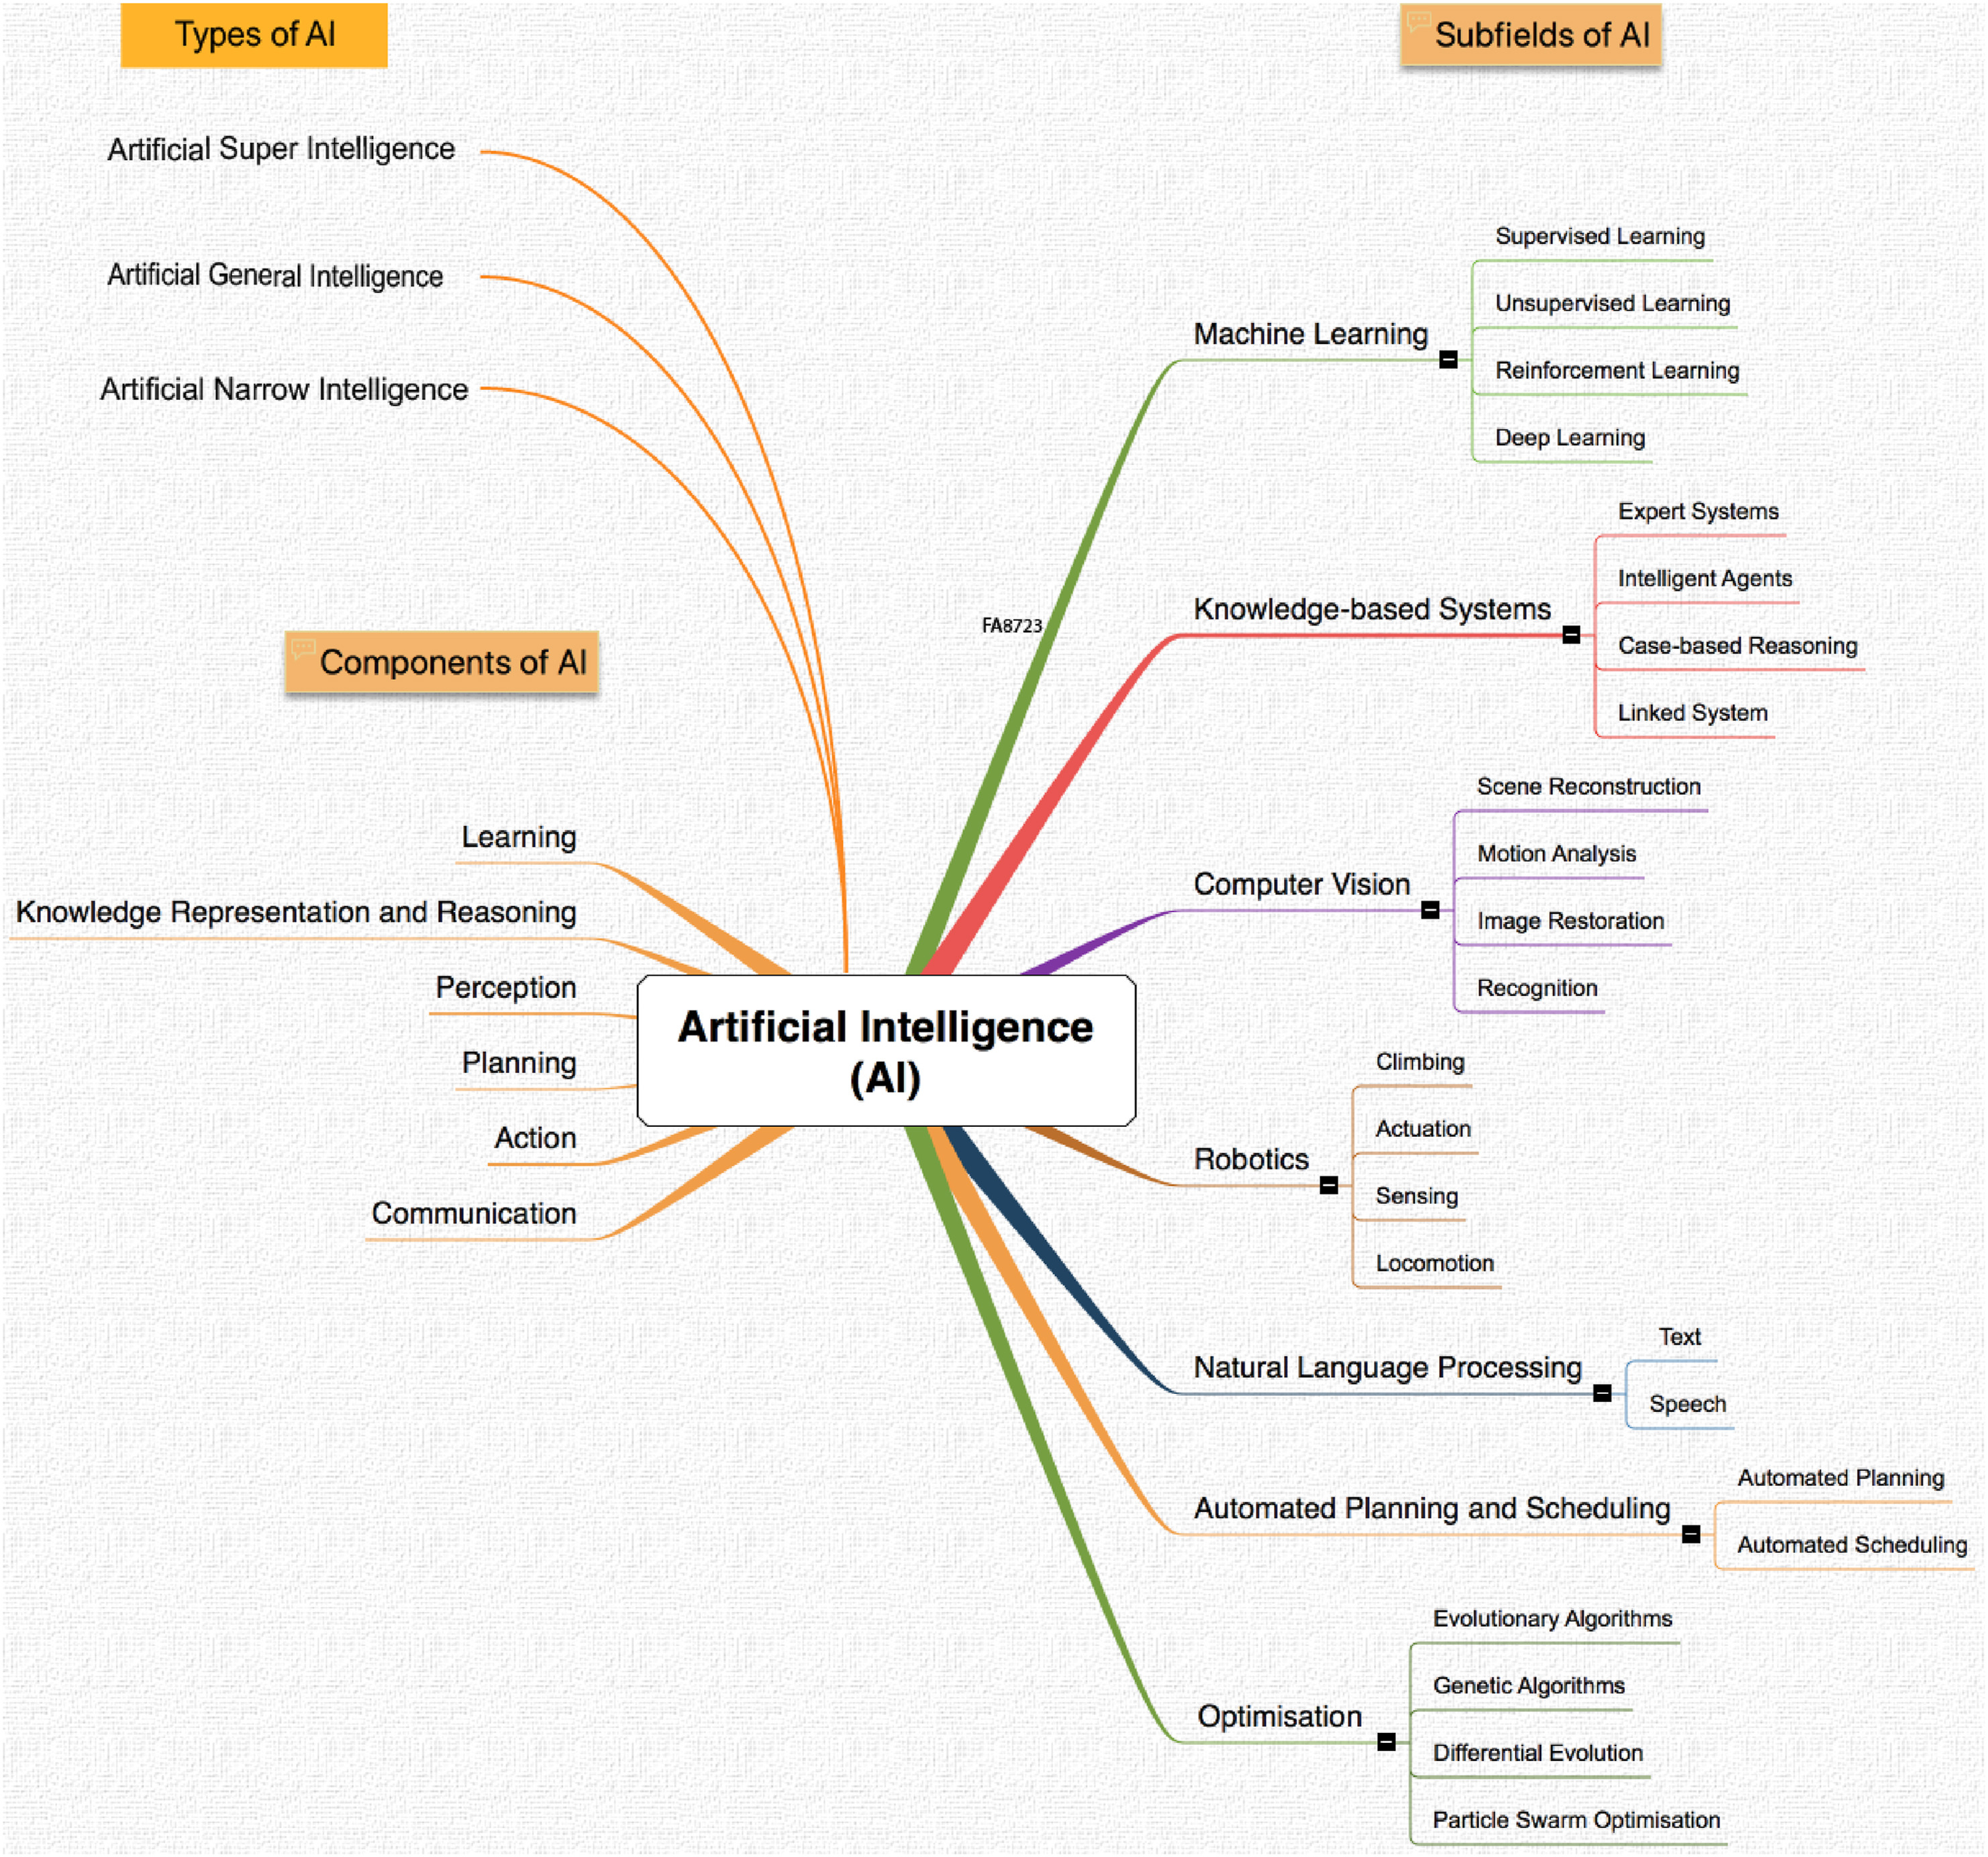
\includegraphics[width=1.1, height=0/96\linewidth]{Images/Artificial Intelligence.jpg}
\caption{اجزاء انواع و زیرشاخه های هوش مصنوعی}
\label{شکل:Artificial Intelligence}
\end{figure}


\subsection{یادگیری ماشین ( Machine Learning )}
یادگیری ماشینی به طراحی و استفاده از برنامه‌های کامپیوتری برای یادگیری از تجربیات یا داده‌های گذشته به منظور مدل‌سازی، کنترل یا پیش‌بینی با استفاده از تکنیک‌های آماری بدون برنامه‌ریزی صریح مربوط می‌شود. روش‌های یادگیری ماشینی عبارتند از: (الف) یادگیری ماشین نظارت شده: این به مطالعه نحوه تصمیم‌گیری ماشین‌ها بر اساس آنچه از مجموعه داده‌های برچسب‌گذاری شده، یعنی جفت‌های ورودی و خروجی دلخواه، آموخته‌اند، مربوط می‌شود. به طبقه بندی و رگرسیون [30] طبقه بندی می شود. (ب) یادگیری ماشینی بدون نظارت: این امر به یادگیری ساختار اساسی در مجموعه داده های بدون برچسب مربوط می شود. آن را به تکنیک های خوشه بندی و کاهش ابعاد [31] و; (C) یادگیری تقویتی (RL): این به عنوان "یادگیری نقشه برداری از موقعیت ها به اقدامات به منظور به حداکثر رساندن یک پاداش اسکالر یا سیگنال تقویت" تعریف می شود [32]. این یک رویکرد محاسباتی است که شامل یادگیری از نتیجه تعاملات با محیط است. و، (د) یادگیری عمیق: این وضعیت فعلی در یادگیری ماشینی است که ثابت کرده است پیش‌بینی‌های دقیق‌تری نسبت به تکنیک‌های یادگیری ماشین معمولی ارائه می‌دهد [[33]، [34]، [35]].

\subsection{بینایی کامپیوتر( Computer Vision )}
بینایی کامپیوتر یک زمینه چند رشته ای است که با شبیه سازی مصنوعی سیستم بینایی انسان سروکار دارد. برای دستیابی به هدف نهایی ساخت ماشین‌هایی که هوش انسانی را تقلید می‌کنند، بینایی کامپیوتر به دنبال این است که با گرفتن تصاویر از طریق دستگاه‌های مناسب، درک سطح بالایی از تصاویر دیجیتالی و چند بعدی، پردازش آنها با استفاده از الگوریتم های پیشرفته و تجزیه و تحلیل تصاویر برای تسهیل تصمیم گیری را فراهم کند.

\subsection{برنامه ریزی و برنامه ریزی خودکار(Automated planning and scheduling )}
برنامه‌ ریزی زیرشاخه‌ ای از هوش مصنوعی است که به توانمندسازی سیستم‌های هوشمند برای دستیابی به اهداف یا مقاصد دلخواه با انتخاب دقیق و توالی اقدامات بر اساس نتایج مورد انتظارشان مربوط می‌شود [36]. برنامه ریزی شامل انتخاب برنامه ها و تخصیص زمان و منابع لازم برای دستیابی به اهداف مورد نظر بر اساس مجموع منابع موجود است [37]. تکنیک‌های برنامه‌ریزی و زمان‌بندی برای ارائه راه‌حل‌هایی برای برنامه‌های پیچیده که بهتر با محدودیت‌های مشکل و نیازهای کاربر تناسب دارند، به کار گرفته می‌شوند [38]. برنامه ریزی به دلیل پیچیدگی، هزینه و زمان مصرف در شرایطی استفاده می شود که منافع آن بیشتر از هزینه باشد [36]. اکتشافی و الگوریتم های رایج مورد استفاده برای برنامه ریزی و زمان بندی شامل تکنیک های جستجو، تکنیک های بهینه سازی و الگوریتم های ژنتیک است.

\subsection{رباتیک}
ربات ها دستگاه های بسیار خودکاری هستند که فعالیت های فیزیکی را در دنیای واقعی انجام می دهند. رباتیک یک فعالیت مهندسی میان رشته ای است که شامل طراحی، ساخت، بهره برداری و نگهداری ربات ها و سایر اقدامات کامپیوتری برای تقلید از اعمال فیزیکی انسان است. ربات‌ها برای کارهای بسیار تخصصی هستند، شکل‌هایی را می‌گیرند که مناسب‌ترین شکل برای استفاده خود هستند و لزوماً شکل انسان‌ نما نیستند، و با استفاده از حسگرها و محرک‌ها با محیط تعامل دارند [18]. [39] اکثر مشکلات یادگیری در رباتیک مشکلات یادگیری ماشینی تقویتی است.

\subsection{سیستم های دانش محور(Knowledge based systems)}
سیستم های مبتنی بر دانش (KBS) شاخه ای از هوش مصنوعی است که با تصمیم گیری ماشینی بر اساس دانش موجود سروکار دارد. اساسا، یک KBS شامل یک پایگاه دانش، یک موتور استنتاج و یک رابط کاربری برای تعامل است. پایگاه دانش از ذخیره دانش تخصصی حوزه، موارد یا تجربیات گذشته یا سایر منابع مرتبط ایجاد می شود. مزیت اصلی آن افزایش بهره وری و کارایی دسترسی آسان و تعامل با دانش بزرگ دامنه مورد نیاز است. KBS استنباط می کند و به نتایجی می رسد که اکتشافی، انعطاف پذیر و شفاف هستند و منطق پشت توصیه های داده شده را در صورت لزوم ارائه می دهند. KBS به (A) سیستم های خبره طبقه بندی می شوند: پایگاه دانش شامل دانش ویژه کار از یک متخصص در یک حوزه خاص برای تقلید از تصمیم گیری در انسان برای حل مشکلات خاص است [40]. (ب) سیستم های استدلال مبتنی بر مورد (CBR): پایگاه دانش سیستم های CBR از تجربیات گذشته یا موارد قدیمی تشکیل شده است که برای توضیح، تفسیر یا نقد موقعیت های جدید استفاده می شود [40]. برای اثربخشی در برخی حوزه‌ها، سیستم‌های CBR باید از دانش تخصصی برای انتخاب موارد مناسب مشابه پروژه جدید استفاده کنند (Juell & Paulson, P., 2003). (ج) سیستم‌های آموزشی هوشمند: این سیستم‌ها از تکنیک‌های هوش مصنوعی استفاده می‌کنند تا به مربیان آنچه را که آموزش می‌دهند، به چه کسانی آموزش می‌دهند و چگونه آن را آموزش می‌دهند، ارائه دهند [41]. و (D) DBMS با رابط های کاربری هوشمند و سیستم های مرتبط: سیستم های پایگاه داده با رابط های کاربری هوشمند هستند که توسط هوش مصنوعی هدایت می شوند. سیستم‌های دستکاری پیوندی یا ابرمتن (HMS) امکان پیمایش آسان از شبکه‌های اطلاعاتی پیچیده را فراهم می‌کنند که نویسندگان و نویسندگان را قادر می‌سازد به راحتی متن‌ها و مراجع را به هم پیوند دهند [42،43].

\subsection{پردازش زبان طبیعی
(Natural Language Processing)}
پردازش زبان طبیعی (NLP) زیرشاخه‌ ای از هوش مصنوعی است که به ایجاد مدل‌ های محاسباتی که توانایی‌ های زبانی انسان‌ها را تقلید می‌کنند، می‌پردازد [44]. NLP در زمینه‌های ترجمه ماشینی، پردازش و خلاصه‌ سازی متن زبان طبیعی، رابط‌ های کاربری، بازیابی اطلاعات چند زبانه و متقابل زبان، تشخیص گفتار و سیستم‌ های خبره کاربرد دارد [45]. وظایف درگیر در NLP عبارتند از برچسب گذاری بخشی از گفتار، تکه تکه کردن، شناسایی موجودیت نامگذاری شده و برچسب گذاری نقش معنایی [46].

\subsection{بهینه سازی}
بهینه ‌سازی مربوط به تصمیم ‌گیری یا انتخاب‌ هایی است که با توجه به مجموعه‌ ای از محدودیت ‌ها، بهترین نتایج را ارائه می‌دهد. به گفته Boyd and Vandenberghe, L., [47]; یک مسئله بهینه سازی ساختاری از مسئله انجام بهترین انتخاب از میان مجموعه ای از انتخاب ها است. بهینه سازی یک پدیده مادام العمر است که در اصل به عنوان یک رشته ریاضی شناخته می شود که به یافتن راه حل بهینه برای هر مسئله ای مربوط می شود. با تولد هوش مصنوعی در دهه 1950، خانواده جدیدی از الگوریتم های فراابتکاری به نام الگوریتم های تکاملی (EA) ایجاد شد [48]. برخی از الگوریتم‌های اخیر متعلق به خانواده EA شامل استراتژی‌های تکاملی (ES)، برنامه‌ریزی تکاملی (EP)، الگوریتم‌های ژنتیک (GA)، تکامل تفاضلی (DE) و بهینه‌سازی ازدحام ذرات (PSO) است [48].

\section{وضعیت هنر و فرصت های آینده کاربردهای هوش مصنوعی در صنعت ساخت و ساز}

\subsection{روند کاربرد هوش مصنوعی در صنعت ساخت و ساز}
شکل 2 به وضوح روند افزایش تعداد انتشارات در حوزه هوش مصنوعی را از دهه 1960 به بعد نشان می دهد. در دهه 1960، استفاده از هوش مصنوعی هنوز در ابتدای راه بود و تعداد بسیار کمی از نشریات از تکنیک های بهینه سازی استفاده می کردند. با گذشت زمان، بهینه‌سازی اصلی‌ترین حوزه مورد علاقه تحقیقاتی در کاربرد زیرشاخه‌های هوش مصنوعی برای صنعت ساخت‌وساز بوده است. این را می توان به مبارزه دیرینه صنعت با سطح بهره وری پایین نسبت داد. بینش دیگری از روندهای تحقیقاتی در طول سال‌ها این است که یادگیری ماشینی در دهه گذشته از سیستم‌های مبتنی بر دانش به عنوان زیرمجموعه مورد علاقه در صنعت ساخت‌وساز پیشی گرفته است. این را می توان به افزایش نیاز به رفع کمبود نیروی کار و مهارت نسبت داد. علاوه بر این، رباتیک همچنین در معرفی پرینت سه بعدی، اسکلت بیرونی، فناوری‌های پهپاد برای فرآیندهای ساخت ‌وساز به صدر کاربردهای هوش مصنوعی در صنعت ساخت‌وساز آمده است (توریز و همکاران، 2017). با این حال، پردازش زبان طبیعی کمترین زمینه تحقیق در صنعت ساخت و ساز بوده است.
بیش از 60 درصد از تحقیقات کاربردی هوش مصنوعی در ساخت و ساز در دهه گذشته انجام شده است و باعث ظهور یا افزایش ظهور فناوری های پیشرفته از جمله: (1) محاسبات کوانتومی شده است. (2) اینترنت اشیا (IoT)؛ (3) امنیت سایبری و (4) بلاک چین. محاسبات کوانتومی این قابلیت را دارد که وظایف محاسباتی خاصی را با کارایی بیشتری نسبت به کامپیوترهای کلاسیک (یا سنتی) حل کند [49،50]. در نتیجه ماهیت خاص اطلاعات کوانتومی، الگوریتم ‌های کوانتومی مؤثرتر از الگوریتم‌های کلاسیک (یا سنتی) هستند. هوش مصنوعی می تواند از قابلیت های محاسبات کوانتومی برای تسریع حل مسئله و بهینه سازی راه حل های آن استفاده کند.
اینترنت از تنها اجازه دادن به انسان ها برای برقراری ارتباط با یکدیگر، به برقراری ارتباط بین چندین اشیا و انسان برای ایجاد یک محیط هوشمند تکامل یافته است [51]. این تحول با پیشرفت‌های اخیر در فناوری مانند حسگرها، محرک‌ها، فناوری‌های بی‌سیم (مانند RFID)، محاسبات ابری، دستگاه‌های سریع‌تر و ارزان‌تر با قابلیت‌های پردازشی افزایش یافته امکان‌پذیر شده است. در صنعت ساخت و ساز، اینترنت اشیاء به طرق مختلف با هوش مصنوعی ادغام شده است، از جمله: صرفه جویی در مصرف انرژی در صورت تقاضا برای نظارت هوشمند انرژی ساختمان [52،53]؛ پلتفرم مدل‌سازی اطلاعات ساختمان (BIM) با قابلیت IoT برای دستیابی به دید و قابلیت ردیابی در زمان واقعی در ساخت‌وسازهای پیش ساخته [54]. و ایجاد هشدارها و آلارم‌های اولیه به عنوان موانع ایمنی دینامیکی برای انرژی خطر در سایت‌های ساخت‌ وساز زیرزمینی (Zhou & Ding، L.Y.، 2017).
مزیت‌ های متعدد ناشی از افزایش دسترسی به اینترنت و سیستم‌های متصل به هم در سراسر جهان، با چالش تهدیدات سایبری در حال تکامل تهدید می‌شود. برخی از نمونه‌هایی از تهدیدات سایبری که در صنعت ساخت‌ وساز رایج هستند عبارتند از بدافزار، مهندسی اجتماعی و فیشینگ [55]. [56] نشان داد که اگرچه صنعت ساخت‌ وساز در یافته‌های مربوط به امنیت سایبری چندان به چشم نمی‌خورد، اما معرفی سطح 3 BIM با اتکای فزاینده به مجازی، قرار گرفتن در معرض جرایم سایبری را افزایش می‌دهد. ادغام روزافزون BIM با داده های سایر منابع خارجی آن را به ویژه در برابر حملات سایبری آسیب پذیر می کند. در واقع، هر فناوری دیجیتالی که در صنعت ساخت ‌وساز استفاده می‌شود، AR/VR، IoT و حتی هوش مصنوعی مانند ربات‌های سخت و نرم، در صورت عدم وجود امنیت شبکه و طرح پاسخ مناسب، در معرض خطر حملات سایبری قرار دارند [57].
از زمان اختراع بلاک چین در سال 2008، رشد سریعی در پذیرش آن وجود داشته است، به ویژه در زمینه ارزهای دیجیتال، مدیریت ریسک، اینترنت اشیا، خدمات عمومی، اجتماعی و مالی (Cearley، [58،59]). فناوری بلاک چین به اطمینان از مشروعیت یک تراکنش، از خرج مضاعف جلوگیری می کند، و با استفاده از رمزنگاری و مکانیزم اجماع برای تأیید [59]، امکان تراکنش های با ارزش بالا را در یک محیط بی اعتماد می کند. ادغام با IOT و BIM برای مدیریت داده ‌های چرخه عمر ساختمان [61] و تقویت زنجیره‌های تامین تولید در صنعت مواد کامپوزیتی هستند [62]. کاربردهای فناوری بلاک چین در صنعت ساخت‌ وساز بی‌اهمیت هستند و این پتانسیل را دارد که بسیاری از موارد را حل کند. مسائل مربوط به اعتماد، ارتباطات و شفافیت در صنعت کاربردهای هوش مصنوعی در ساخت و ساز را می توان با فناوری بلاک چین برای توسعه راه حل هایی که امن، شفاف و دارای CDE غیرمتمرکز هستند ادغام کرد. 

\begin{figure}[t]
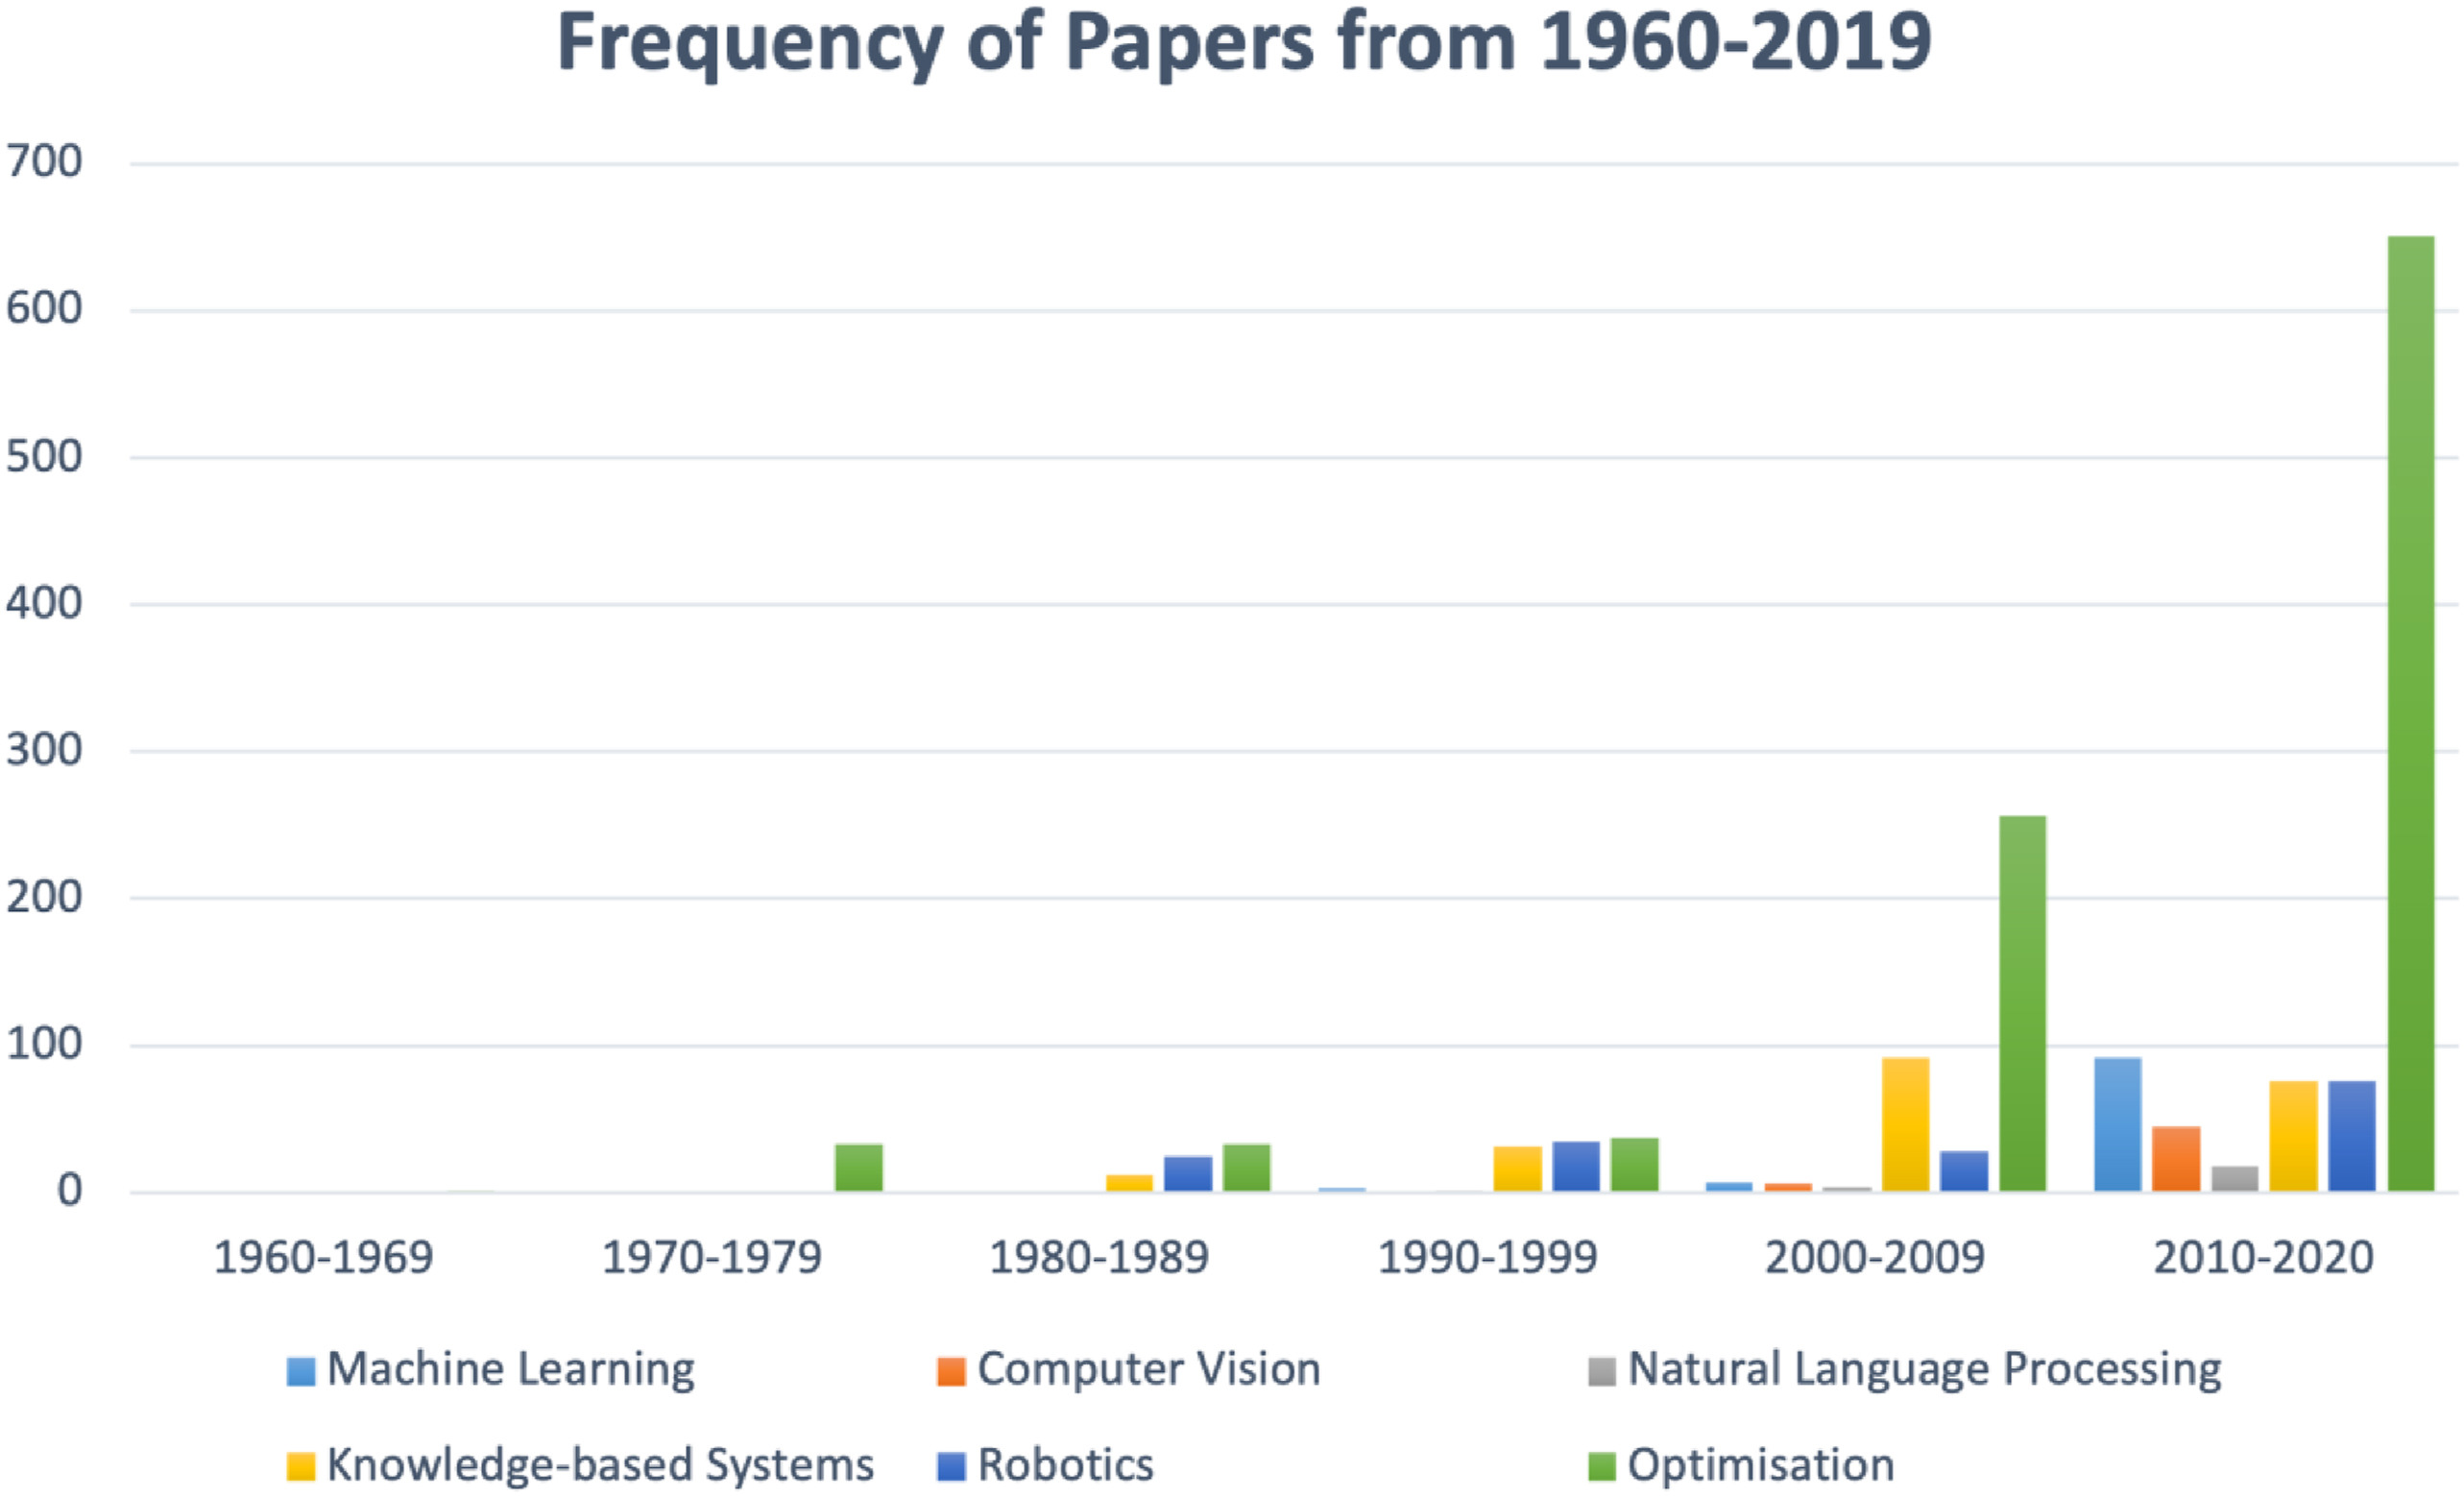
\includegraphics[width=1, height=1\linewidth]{Images/Frequency Of Paper.jpg}
\caption{مقاله های انتشار یافته از 1960 تا 2019}
\label{شکل:Frequency Of Paper}
\end{figure}


\subsection{کاربرد زیرشاخه های هوش مصنوعی در صنعت ساخت و ساز}
شکل 1 برخی از مزایا و محدودیت های زیرشاخه های هوش مصنوعی در صنعت ساخت و ساز را نشان می دهد. مزایای مشابه در همه زیر شاخه ها شامل افزایش هزینه و صرفه جویی در زمان، بهبود ایمنی، دقت بهتر و افزایش بهره وری کلی است. برخی از محدودیت ‌های زیرشاخه‌های هوش مصنوعی در ساخت ‌وساز شامل داده‌های ناقص، هزینه اولیه بالای استقرار، داده‌ها و مسائل مربوط به کسب دانش است.

\subsection{زمینه های کاربردی مشترک و فرصت های آینده هوش مصنوعی در ساخت و ساز}
حوزه های شناسایی شده کاربرد هوش مصنوعی در صنعت ساخت و ساز، پیشرفته ترین و فرصت های بالقوه آینده برای افزایش پذیرش هوش مصنوعی را ارائه می دهد. از جدول، چهارده (14) زیر دامنه با کاربردهای پیشرفته مرتبط و فرصت‌های بالقوه برای مسائل خاص ساخت و ساز شناسایی شدند. برخی از زیر دامنه های شناسایی شده شامل بهینه سازی منابع و ضایعات است. خدمات ارزش محور؛ مدیریت زنجیره تامین؛ سلامت و ایمنی، تجزیه و تحلیل قرارداد ساخت و ساز مبتنی بر هوش مصنوعی؛ رابط های کاربر صوتی؛ و سیستم حسابرسی مبتنی بر هوش مصنوعی برای امور مالی ساخت و ساز. تحت خدمات ارزش محور، زیردامنه هایی مانند برآورد و زمان بندی، تجزیه و تحلیل سایت ساخت و ساز، ایجاد شغل، هوش مصنوعی و ادغام BIM با سایر ابزارهای صنعت 4.0 مانند اینترنت اشیا (IoT) توضیح داده شده است.

\subsubsection{بهینه سازی منابع و ضایعات}
به دلیل توسعه مداوم و سریع، هر ساله مقدار فزاینده ای از زباله های ساخت و ساز و تخریب (C&DW) تولید می شود [102,103]. این فعالیت های      ساختمانی اثرات نامطلوبی بر محیط زیست، منابع طبیعی و انسانی در سطح جهان دارند [103]. [104] یک تغییر پارادایمیک در رویکردهای مدیریت پسماند از هوشمندی زباله مشاهده کرد، که اقداماتی را برای کاهش ضایعات تنها پس از وقوع، به رویکردهای پیشگیرانه مبتنی بر داده، یعنی تجزیه و تحلیل زباله (WA)، که ضایعات را از طریق طراحی به حداقل می‌رساند، پیشنهاد می‌کند. استفاده فزاینده ای از BIM به عنوان یک محیط مجازی، کم هزینه و محاسباتی برای فعال کردن طراحی ساخت و ساز با هدف به حداقل رساندن تولید زباله وجود داشته است [72،74]. [71] پتانسیل تکنیک های تجزیه و تحلیل داده های پیشرفته برای تولید پروفایل های تولید زباله با جزئیات بیشتر را برجسته می کند. بنابراین، استفاده از تجزیه و تحلیل داده های پیشرفته می تواند ضایعات را به طور گسترده به حداقل برساند.
تجزیه و تحلیل زباله به داده های متنوعی از منابع مختلف مانند طراحی ساختمان، خواص مصالح و استراتژی های ساخت و ساز بستگی دارد که امکان محاسبات با کارایی بالا و پردازش در زمان واقعی را فراهم می کند [104,105]. حجم زیاد داده ها نیازمند تکنیک های پیشرفته تجزیه و تحلیل داده است تا آن ها را به اطلاعات مرتبط با حداقل سازی زباله تبدیل کند. این امر مستلزم اتخاذ تکنیک های هوش مصنوعی برای مدیریت موثر زباله است [106,107]. به ویژه، استفاده از تکنیک‌های پیشرفته هوش مصنوعی با BIM برای بهینه‌سازی طراحی برای ساخت و ساز خارج از سایت، انتخاب مواد، استفاده مجدد و بازیابی، تدارکات کم مصرف، ساختارشکنی و انعطاف‌پذیری. جدول 3 به طور خلاصه فرصت های پیشرفته و بالقوه برای این زیر دامنه را نشان می دهد.

\subsubsection{خدمات ارزش محور}
این بخش طیف گسترده ای از خدمات غیر اصلی را مورد بحث قرار می دهد که می تواند از روند نوظهور هوش مصنوعی در صنعت ساخت و ساز بهره مند شود.

\begin{itemize}
\item
\textbf{\emph{برآورد و زمان بندی:}}
\\مدل های تخمین (یا پیش بینی) مبتنی بر هوش مصنوعی کاربرد گسترده ای در حوزه های مختلف صنعت ساخت و ساز دارند. به ویژه، این مدل‌های تخمین در پیش‌بینی اولیه هزینه و مدت ساخت و ساز، که عوامل کلیدی موفقیت پروژه هستند، مفید هستند (Sridarran, 2017). برآورد هزینه و زمان غیرقابل اعتماد پروژه می تواند پیامدهای اقتصادی و مالی بزرگی داشته باشد (Flyvbjerg et al., 2002).
BIM آخرین وضعیت فعلی در صنعت ساخت و ساز است که برای افزایش قابلیت اطمینان تخمین هزینه و زمان در صنعت ساخت و ساز استفاده می شود [75,108]. ادغام زمان (4 بعدی) و هزینه (5 بعدی) با BIM، برنامه ریزی بهتر در مراحل اولیه طراحی برای برنامه ریزی پروژه و برآورد هزینه را امکان پذیر می کند (Jrade & Lessard, 2015؛ McCuen, 2018). با این وجود، علی‌رغم مزایای عظیم BIM، شواهد همچنین نشان داده‌اند که مزیت اتوماسیون ناشی از BIM تنها اطلاعات موجود در مدل را در نظر می‌گیرد در حالی که به ترتیب عوامل ذهنی خارجی، مواد اضافی و منابع را نادیده می‌گیرد (Golaszewska و Salamak، 2017). در نتیجه، استفاده از BIM برای برآورد هزینه و زمان هنوز به کار زیادی برای برآوردگر هزینه نیاز دارد.
این امر مستلزم ادغام تکنیک های پیشرفته هوش مصنوعی مانند یادگیری عمیق با BIM برای پیش بینی هزینه و زمان برای استفاده از دقت بهتر است. در نتیجه، تکنیک‌های یادگیری عمیق همچنین می‌توانند به پیش‌بینی بهتر عوامل مرتبط دیگر مانند ورشکستگی، موفقیت، انرژی، کارایی کربن و حتی اتلاف کمک کنند.

\item
\textbf{\emph{تجزیه و تحلیل سایت ساختمانی:}}
\\سایت های ساختمانی به دلیل فراگیر شدن فزاینده حسگرهای IoT و سایر فناوری های دیجیتال به سرعت در حال تبدیل شدن به محیط های کاری هوشمند هستند [109]. تجزیه و تحلیل سایت ساخت و ساز مربوط به تولید، جمع آوری، ذخیره سازی و تجزیه و تحلیل داده های سایت ساخت و ساز برای ایجاد بینش عمیق برای تجسم است [109]. حجم زیادی از تصاویر، ویدئوها و سایر اشکال داده در سایت‌های ساخت‌وساز مانند گزارش‌ها، تجهیزات بلادرنگ و نظارت بر سایت تولید می‌شوند که عمدتاً ساختاری ندارند. داده‌های جمع‌آوری‌شده را می‌توان در BIM جمع‌آوری کرد و با استفاده از تکنیک‌های پیشرفته هوش مصنوعی برای بهینه‌سازی عملکرد سایت در تمام زمینه‌های کلیدی مانند برنامه‌ریزی، طراحی، ایمنی، کیفیت، زمان‌بندی و هزینه تجزیه و تحلیل کرد [110].
لین و گل پرور فرد [76] یک پایه نظری برای داده های بصری و تجزیه و تحلیل پیش بینی برای کنترل پروژه فعال در سایت های ساخت و ساز ارائه کردند [77]. پتانسیل داده های بصری بزرگ و BIM برای مدل سازی تجزیه و تحلیل عملکرد ساخت و ساز را مورد بحث قرار داد. شواب و همکاران [78] فرآیند دیجیتالی کردن فرآیند برنامه ریزی چیدمان سایت ساخت و ساز در BIM را با استفاده از بررسی مدل مبتنی بر قانون تشریح کرد. نیاز به توسعه یک ابزار تجزیه و تحلیل سایت جامع با استفاده از هوش مصنوعی برای تجزیه و تحلیل زمان واقعی و مبتنی بر ابر داده های تولید شده در سایت ساخت و ساز وجود دارد. این باعث بهبود بهره وری، کنترل کیفیت و کمک به دستیابی به اهداف تعیین شده عملکرد می شود. یک چت ربات هوش مصنوعی سایت ساخت و ساز برای دریافت به روز رسانی در زمان واقعی در مورد فعالیت های سایت، برای مدیران پروژه و سایر ذینفعان مرتبط بسیار مفید خواهد بود.

\item
\textbf{\emph{ایجاد شغل:}}
\\مشاغل ساختمانی سومین مشاغل در معرض خطر اتوماسیون در دهه آینده هستند [81]، به دلیل رواج فزاینده فناوری های اتوماسیون مانند هوش مصنوعی و IoT. اکثر مشاغل ساختمانی که به تحصیلات متوسط تا پایین نیاز دارند در معرض خطر بالای (38-45٪) اتوماسیون تا اواسط دهه 2030 قرار دارند [81]. با این حال، پذیرش چنین فناوری‌هایی می‌تواند به ایجاد نقش‌های کاملاً جدید برای جذب و مهارت مجدد کارگران آواره در صنعت منجر شود. به عنوان مثال، ظهور BIM منجر به ایجاد نقش های جدیدی مانند مدیر پروژه BIM، مدیر، هماهنگ کننده و طراح شده است [79]. پذیرش فناوری‌های دیجیتالی مانند هوش مصنوعی در صنعت ساخت‌وساز باعث ایجاد انواع جدیدی از مشاغل مانند محقق، مربی و مهندس هوش مصنوعی ساختمانی می‌شود. محققان مسئول رساندن صنعت ساخت و ساز به مرز پذیرش هوش مصنوعی با انجام مداوم تحقیقات و آوردن نوآوری در این بخش خواهند بود. مهندسان هوش مصنوعی ساخت و ساز بر توسعه و استقرار راه حل های پیشرفته هوش مصنوعی متناسب با صنعت ساخت و ساز تمرکز خواهند کرد. در نهایت، مربیان و آزمایشگران برای اطمینان از اینکه این راه حل ها مانند ربات ها و عوامل مستقل اهداف تعیین شده را به طور موثر و کارآمد انجام می دهند، مورد نیاز خواهند بود. به عنوان مثال، کارگران با مهارت کم تا متوسط که شغل خود را به دلیل اتوماسیون از دست می دهند، می توانند به عنوان مربی و آزمایش کننده برای سیستم هایی که جایگزین آنها می شوند، عمل کنند.

\item
\textbf{\emph{هوش مصنوعی و BIM با ابزارهای صنعت:}}
\\BIM آخرین وضعیت فعلی در صنعت معماری، مهندسی و ساخت و ساز (AEC) است که در سراسر جهان پذیرفته شده است [111]. به عنوان مثال، دولت بریتانیا سطح 2 BIM را برای تمام پروژه‌هایی که به صورت عمومی خریداری می‌شوند الزامی کرد. با این حال، علیرغم تلاش برای تبدیل BIM به عنوان استاندارد واقعی در سطح جهانی، نرخ پذیرش آن هنوز بسیار پایین است [112]. در نتیجه، انجام تحقیقات مرتبط در مورد راه‌های بهبود پذیرش BIM مهم است. به عنوان مثال، برخی از مطالعات، برنامه های کاربردی BIM را با زیرشاخه های هوش مصنوعی مانند NLP برای بهبود ناوبری رابط های BIM ترکیب کرده اند. با توجه به مطالعه کار پروژه ساخت و ساز انجام شده توسط Styhre و همکاران. (2006)، نویسندگان استدلال کردند که ماهیت عملکرد ساخت و ساز تا حد زیادی به ارتباطات مستقیم کلامی و نمادین برای به اشتراک گذاشتن تخصص و اطلاعات وابسته است. شاید، این ممکن است به این دلیل باشد که بدون شک گفتار یکی از قدیمی‌ترین و طبیعی‌ترین شکل‌های ارتباطی است (Dutoi, 1997; Furui et al., 2004; Taylor, 2009). ادغام تعامل صوتی با BIM باعث می شود احساس طبیعی تر و صادقانه تر به ماهیت ساخت و ساز داشته باشید. مطالعات دیگر همچنین هوش مصنوعی و BIM را با سایر ابزارهای صنعت 4.0 مانند اینترنت اشیا (IoT) (Zhou & Ding, L.Y., 2017)، شهرهای هوشمند [84]، واقعیت افزوده [87]، بلاک چین [60] و محاسبات کوانتومی ترکیب کرده اند. [50]

\end{itemize}

\subsubsection{مدیریت زنجیره تامین (SCM)}
مطالعه اخیر توسط لو و همکاران. [113]، برای کشف عوامل مؤثر بر تعالی و نتایج زنجیره تأمین، موضوعاتی مانند آموزش دانش SCM و فرهنگ زنجیره تأمین را آشکار کرد. موانع اصلی یافت شده فقدان خرید در سطح بالا و درک کلی از زنجیره تامین است. ادبیات همچنین نشان داد که هزینه بالای فناوری اطلاعات پیشرفته برای SCM، فقدان چارچوب‌های اندازه‌گیری عملکرد خاص و منحصربه‌فرد، فقدان اعتماد سازمانی و کانال‌های ارتباطی مؤثر بین شرکا یک عامل مانع اصلی بوده است [114,115]. تکنیک های هوش مصنوعی می توانند نقش مهمی در حل این مسائل ایفا کنند که مانع تعالی در زنجیره تامین می شوند.
تسانگ و همکاران [89] یک سیستم پایش ریسک بلادرنگ مبتنی بر اینترنت اشیا را برای کنترل کیفیت محصول و خطرات ایمنی شغلی در زنجیره های سرد با استفاده از شبکه حسگرهای بی سیم، خدمات پایگاه داده ابری و منطق فازی توسعه داد. به گفته باراتا و همکاران. [90]؛ ادغام بلادرنگ زنجیره های تامین غیرمتمرکز در راس دستور کار موسسات اروپایی، صنایع و شرکت های مشاوره چندملیتی قرار دارد. شیونگ و همکاران [91] یک زبان مشخصات فرآیند را برای بهبود ارتباطات زنجیره تامین برای ساخت و ساز خارج از سایت توسعه داد.
این مطالعه خواستار توسعه یک سیستم مدیریت دانش و نظارت بر زنجیره تامین غیرمتمرکز است. مزایای بلاک چین برای اطمینان از شفافیت و مشروعیت تراکنش ها، همراه با تجزیه و تحلیل های پیشرفته با استفاده از هوش مصنوعی، این پتانسیل را دارد که اعتماد سازمانی و مسائل ارتباطی در زنجیره تامین ساخت و ساز را حل کند. برای مثال، موندراگون و همکاران. [62] کاربرد بلاک چین را برای افزایش زنجیره تامین تولید بررسی کرد و نتایج نشان می‌دهد که تاریخچه تولید و ذخیره‌سازی محصول بدون دستکاری است. هوش مصنوعی می تواند برای مدیریت کل فرآیند زنجیره تامین برای شناسایی مشکلات احتمالی و اطمینان از تحویل به موقع و با کیفیت پروژه استفاده شود. همچنین، ایجاد چت ربات های هوش مصنوعی برای سیستم مدیریت زنجیره تامین برای مهار اطلاعات مربوطه به روشی ساده.

\subsubsection{تجزیه و تحلیل سلامت و ایمنی}
تجزیه و تحلیل سلامت و ایمنی (HSA) از تکنیک های پیشرفته تجزیه و تحلیل داده ها برای پیش بینی و جلوگیری از حوادث شغلی در محل کار استفاده می کند. صنعت ساخت و ساز نسبت به سایر صنایع به میزان قابل توجهی بالاتر از صدمات و مرگ و میر شغلی را ثبت می کند [116]. این امر به این دلیل است که کار ساخت و ساز به دلیل خطرات در محل مانند کار از ارتفاع، گرفتار شدن، افتادن اشیا، تجهیزات و ابزار، گرد و غبار و مواد سمی و از دست دادن شنوایی به دلیل سر و صدا بسیار خطرناک است [110]. این خطرات می تواند منجر به مشکلات سلامتی طولانی مدت، ناتوانی یا حتی مرگ کارگران شود [117]. برای کارفرمایان، این می تواند به معنای از دست دادن شهرت، کاهش بهره وری، افزایش حق بیمه، دعاوی حقوقی و هزینه های خسارت باشد. از این رو، نیاز به اتخاذ رویکردی پیشگیرانه با استفاده از فناوری های دیجیتالی مانند هوش مصنوعی برای پیش بینی حوادث یا خطرات سلامتی قبل از وقوع و پیشگیری از آنها است.
برخی از کاربردهای اخیر هوش مصنوعی در سلامت و ایمنی شامل شناسایی و پیشگیری از خطر سقوط مبتنی بر BIM است [92]. ادغام فناوری های مبتنی بر حسگر با BIM برای بهبود ایمنی ساخت و ساز [94،95]؛ و فناوری پوشیدنی مورد استفاده در نظارت بر ایمنی ساخت و ساز [93]. 
بر اساس موارد ذکر شده، می توان استنباط کرد که داده های فناوری های دیجیتال مختلف مانند حسگرهای IoT، UAV و دستگاه های پوشیدنی در مراحل مختلف ساخت و ساز با BIM برای جلوگیری و کاهش خطرات ایمنی استفاده می شود. این موارد ناگزیر نیاز به استفاده از تکنیک‌های پیشرفته هوش مصنوعی (مانند یادگیری عمیق) برای استفاده مرتبط از این داده‌ها برای مدیریت ایمنی پیش‌بینی‌کننده و فعال دارد. وینگ و همکاران [116] هفت عامل متداول را که باعث بروز حوادث ساختمانی می شوند، شامل اقدامات کارگر، مدیریت ریسک، نظارت فوری، قابلیت استفاده از مواد یا تجهیزات، خطرات محلی، قابلیت های کارگر و مدیریت پروژه شناسایی کرد. همه این عوامل پتانسیل حل شدن با استفاده از فناوری‌های هوش مصنوعی مانند روباتیک، بینایی کامپیوتر، تجزیه و تحلیل داده‌های پیشرفته و تکنیک‌های بهینه‌سازی را دارند، به‌ویژه زمانی که با سایر فناوری‌های دیجیتال ادغام شوند. همچنین، فرآیند مدیریت بهداشت و ایمنی از یک سیستم جامع تر که نظارت، تجسم، اطلاع رسانی و اقدام را یکپارچه می کند، بهره مند خواهد شد.

\subsubsection{درک قرارداد ساخت و ساز مبتنی بر هوش مصنوعی}
مدیریت قرارداد ساخت و ساز می تواند بسیار پیچیده باشد، شامل قراردادهای حجیم و متعدد که در آن اشتباهات اغلب پیامدهای بزرگی دارند [96]. برخی از این پیامدها شامل هزینه های دادرسی، دعاوی، تاخیر پروژه و از دست دادن شهرت است. یک چالش اصلی این است که مدیریت قرارداد فعلی به شدت به انسان هایی مانند مدیران قرارداد یا تیم حقوقی وابسته است، که آن را مستعد خطا و اشتباه می کند. این امر مستلزم اتوماسیون مدیریت قرارداد با هوش مصنوعی است تا تلاش‌های مدیران قرارداد یا تیم‌های حقوقی را با اطمینان از سریع‌تر و دقیق‌تر بودن فرآیندها افزایش دهد [118]. این امر امکان استعلام آسان قراردادها را برای بازیابی اطلاعات مربوطه، خلاصه قرارداد، تهیه پیش نویس قراردادها، شناسایی بندهای مستعد اختلاف، مذاکره قرارداد و حل اختلاف، قرارداد، تعهدات، اجرا و بسته شدن را فراهم می کند.
یکی از چالش‌های اصلی توسعه ابزار مبتنی بر هوش مصنوعی برای مدیریت قرارداد، اجرای خلاصه‌سازی متن است که برای بازیابی اطلاعات مختصر اما مهم از قراردادها لازم است. این یک کار دشوار است که توجه محققان را می طلبد زیرا قراردادهای ساخت و ساز با قراردادهای عمومی متفاوت است و به همین دلیل مستلزم آموزش خاص ساخت و ساز است. چالش دیگر، درک مطلب خواندن ماشینی (MRC) است که توانایی رایانه‌ها برای درک یک متن داده شده، فرمول‌بندی سؤالات علیه آن و ایجاد پاسخ‌های خوب است. MRC یک کار بسیار چالش برانگیز است که محققان به شدت روی آن کار می کنند. چندین مجموعه داده خاص برای برخی از دامنه‌ها وجود دارد که برای محک زدن و آموزش مدل‌های MRC در دسترس عموم قرار گرفته‌اند. MS MARCO [119]، NewsQA [120]، SearchQA. با این حال، هیچ مجموعه داده ای منحصر به فرد برای صنعت ساخت و ساز وجود ندارد که برای آموزش مدل های MRC ساخت و ساز ضروری است. این فرصتی برای تحقیقات بیشتر است که می تواند MRC را در ساخت و ساز و در نهایت مدیریت قرارداد بهبود بخشد.

\subsubsection{رابط های کاربری صوتی}
ماهیت پرمشغله و مشغله چشمی کار ساخت و ساز باعث می شود رابط های کاربر با قابلیت صوتی (VUI) جایگزین مناسبی برای حالت های فعلی ارتباط با دستگاه ها در سایت های ساخت و ساز باشد [99]. کارگران ساختمانی اغلب مجبورند با برنامه های نرم افزاری مانند BIM در محل ساخت و ساز ارتباط برقرار کنند، اما تایپ کردن دستگاه ها برای بازیابی اطلاعات می تواند منجر به خطرات ایمنی شود. این امر باعث شده است که سایر وسایل ارتباطی با ابزارهای دیجیتالی مانند گفتار مورد توجه قرار گیرد. این امر با افزایش محبوبیت رابط های کاربری با قابلیت گفتار که گاهی اوقات به عنوان دستیارهای خودکار به کار می روند، تقویت می شود. الکسا، سیری، کورتانا [121]. یافته‌های این    مطالعه نشان می‌دهد که گفتار در تحقیقات ساخت‌وساز توجه زیادی از سوی محققان به خود جلب نکرده است.
با وجود اینکه اخیراً پیشرفت‌های زیادی در VUI صورت گرفته است، استفاده از آن هنوز به دلیل برخی چالش‌ها، به‌ویژه چالش‌های خاص در صنعت ساخت‌وساز، مانع می‌شود. یکی از چالش های اصلی این است که مکان های  
ساخت و ساز معمولاً بسیار پر سر و صدا هستند [122] که اطلاعات ناخواسته را در سیگنال گفتار قرار می دهد. این می تواند خطاهای بسیار زیادی ایجاد کند که ممکن است کاربران را ناامید کند و در نهایت منجر به عدم تداوم استفاده شود. چالش های دیگر عبارتند از تنوع بلندگو، بهبود صدا، همفون، ابهام، مقدار داده و فضای جستجو. حل این چالش ها به طور بالقوه می تواند منجر به استفاده یکپارچه از VUI در صنعت ساخت و ساز شود. برای این منظور، توسعه یک مجموعه داده قوی از دستورات صوتی رایج در موقعیت های مختلف در سایت ساخت و ساز باید جمع آوری شود. این را می توان برای آموزش مدل های برنامه صوتی ساخت و ساز استفاده کرد. 

\subsubsection{سیستم حسابرسی مبتنی بر هوش مصنوعی برای امور مالی ساخت و ساز}
علی رغم خروجی های اقتصادی عظیم تولید شده توسط صنعت ساخت و ساز، نرخ ورشکستگی شرکت ها هنوز بسیار بالا است [123]. این ممکن است تا حدی به این دلیل باشد که اکثر مشاغل ساختمانی مدیریت مالی خود را به دلیل منحصر به فرد بودن و طولانی بودن مدت پروژه ها که برای موفقیت پروژه بسیار مهم است، دشوار می دانند [124]. شرکت‌های ساختمانی اغلب پروژه‌های متعددی دارند که به طور همزمان شامل جابه‌جایی کارکنان و تجهیزات بین پروژه‌ها می‌شود [125]، با حاشیه سود ناچیز به دلیل مناقصه رقابتی و هزینه‌های سربار که به درستی محاسبه نشده است [126]. از این رو، مهم است که اطمینان حاصل شود که پروژه ها و هزینه های سربار عمومی به طور موثر پیگیری می شوند [127]. تمرکز نه تنها باید بر ارائه کار با کیفیت، بلکه مدیریت فعال منابع مالی باشد [128]. در حال حاضر، هیچ ابزار حسابرسی مالی مبتنی بر هوش مصنوعی برای ردیابی موثر هزینه‌های پروژه و پیش‌بینی مشکلات مالی بالقوه قبل از وقوع وجود ندارد [129]. بر این اساس، مدیران مالی   می توانند زمانی که یک پروژه بیش از حد یا کمتر از آن خرج می کند، فعالانه پاسخ دهند و تأثیر کلی آن را بر سایر پروژه ها و کل تجارت در زمان واقعی اندازه گیری کنند. این امر تصمیمات ذینفعان شرکت را هدایت می کند و شرکت را از ورشکستگی نجات می دهد.

\section{چالش ها}
تاکنون، این مطالعه فرصت ها و همچنین روندهای نوظهور در کاربرد هوش مصنوعی در فرآیندهای ساخت و ساز را شناسایی کرده است. برای تقویت بیشتر این حوزه از دانش، شناسایی و بحث در مورد چالش های کلیدی مهم است. شکل 3 فرصت ها، روندهای نوظهور، چالش ها و مسائل تحقیقاتی باز هوش مصنوعی در صنعت ساخت و ساز را نشان می دهد. شش حوزه چالش اصلی موثر بر پذیرش هوش مصنوعی در ساخت و ساز عبارت است از:

\subsection{مسائل فرهنگی و هوش مصنوعی قابل توضیح 
( Cultural Issues and Explainable AI )}
این یک واقعیت شناخته شده است که صنعت ساخت و ساز یکی از صنایع کم دیجیتالی است و در پذیرش فناوری های جدید کند است [1]. این می تواند به دلیل ماهیت مخاطره آمیز و پرهزینه بیشتر فرآیندهای ساخت و ساز باشد، جایی که اشتباهات کوچک اغلب پیامدهای بزرگی دارند. در ساخت‌وساز، روش‌های سنتی انجام کارها بیش از فناوری‌های جدید اما غیرقابل اعتماد که وعده ارائه پاداش‌های بزرگ را می‌دهند، ترجیح داده می‌شوند (Babič & Rebolj, 2016). این بدان معنی است که صنعت ساخت و ساز در پذیرش فناوری های نوآورانه کند است. برخلاف بخش‌هایی مانند تولید، سایت‌های ساخت‌وساز عمدتاً منحصربه‌فرد و متفاوت هستند که به هوش مصنوعی نیاز دارد که بتواند سریعاً در محیط‌های متغیر یاد بگیرد و سازگار شود. این بدان معناست که فناوری‌های هوش مصنوعی برای به کارگیری در صنعت ساخت‌وساز باید در پروژه‌ها یا سایت‌های مختلف ساختمانی قابل استفاده باشند و کاملاً آزمایش شوند تا پیمانکاران و مشاغل ساختمانی را متقاعد کنند که از آنها استفاده کنند. این ممکن است شامل بهره گیری از سایر فناوری های دیجیتال مانند بلاک چین برای بهبود اعتماد و شفافیت باشد. علاوه بر این، بیشتر سیستم‌های یادگیری ماشینی از رویکرد جعبه سیاه پیروی می‌کنند، به این معنی که دلایل رسیدن به نتیجه‌گیری را توضیح نمی‌دهند. برای ایجاد اعتماد در چنین سیستم هایی، برای متخصصان ساخت و ساز ضروری است که بدانند سیستم چگونه تصمیم می گیرد. به این ترتیب، این امر مستلزم استفاده از هوش مصنوعی قابل توضیح (XAI) برای تولید مدل‌های قابل توضیح است و انسان‌ها را قادر می‌سازد تا سیستم‌ها را درک، اعتماد و مدیریت کنند. برخی از رویکردهای محبوب XAI شامل توضیحات مدل-آگنوستیک محلی قابل تفسیر (LIME) [130] و انتشار ارتباط لایه ای (LRP) [131] است.

\subsection{امنیت}
علی رغم توانایی هوش مصنوعی برای تقویت امنیت و شناسایی نفوذها [132]، همچنین هدف اصلی برای بهره برداری توسط هکرها، جرایم سایبری و نفوذ به حریم خصوصی است. این یک موضوع مهم با پیامدهای اقتصادی و مالی عظیم است. اشتباهات کوچک در فرآیندهای ساخت و ساز اغلب منجر به پیامدهای کیفیت، هزینه و زمان بسیار زیادی می شود، با یک اثر جابجایی بر برنامه کلی پروژه (زمان، هزینه، زنجیره تامین و تدارکات، تدارکات، و غیره) [133]. مهمتر از همه، ایمنی کارگران ساختمانی ممکن است به خطر بیفتد که می تواند منجر به حوادث تهدید کننده زندگی یا تلفات جانی شود. به عنوان مثال، یک سیستم بینایی رایانه ای که تجهیزات ساخت و ساز خودکار را شناسایی می کند، ممکن است فریب بخورد تا به کارگر ساختمانی که در ارتفاع کار می کند برچسب غلط بزند. استفاده از هوش مصنوعی برای کنترل کامل برخی فرآیندها یا تقویت فعالیت های کارگران ساختمانی باید با حداقل خطرات امنیتی یا بدون خطرات امنیتی انجام شود. این امر مستلزم استراتژی‌های کاهشی مانند استفاده از یادگیری ماشینی متخاصم است. یادگیری ماشین متخاصم (ML) مطالعه تکنیک های یادگیری ماشین موثر در برابر حریف متخاصم است [134]. استفاده از ML متخاصم از دیدگاه دفاع امنیتی و نیاز به طراحی الگوریتم هایی که می توانند در برابر حملات سطح بالا مقاومت کنند، نشات می گیرد. همچنین، تحقیقات بیشتری در این زمینه باید انجام شود، به ویژه برای فناوری هایی که در حال ظهور برای تحقیقات ساخت و ساز مانند بینایی کامپیوتر و روباتیک هستند.


\begin{figure}[h]
\centering
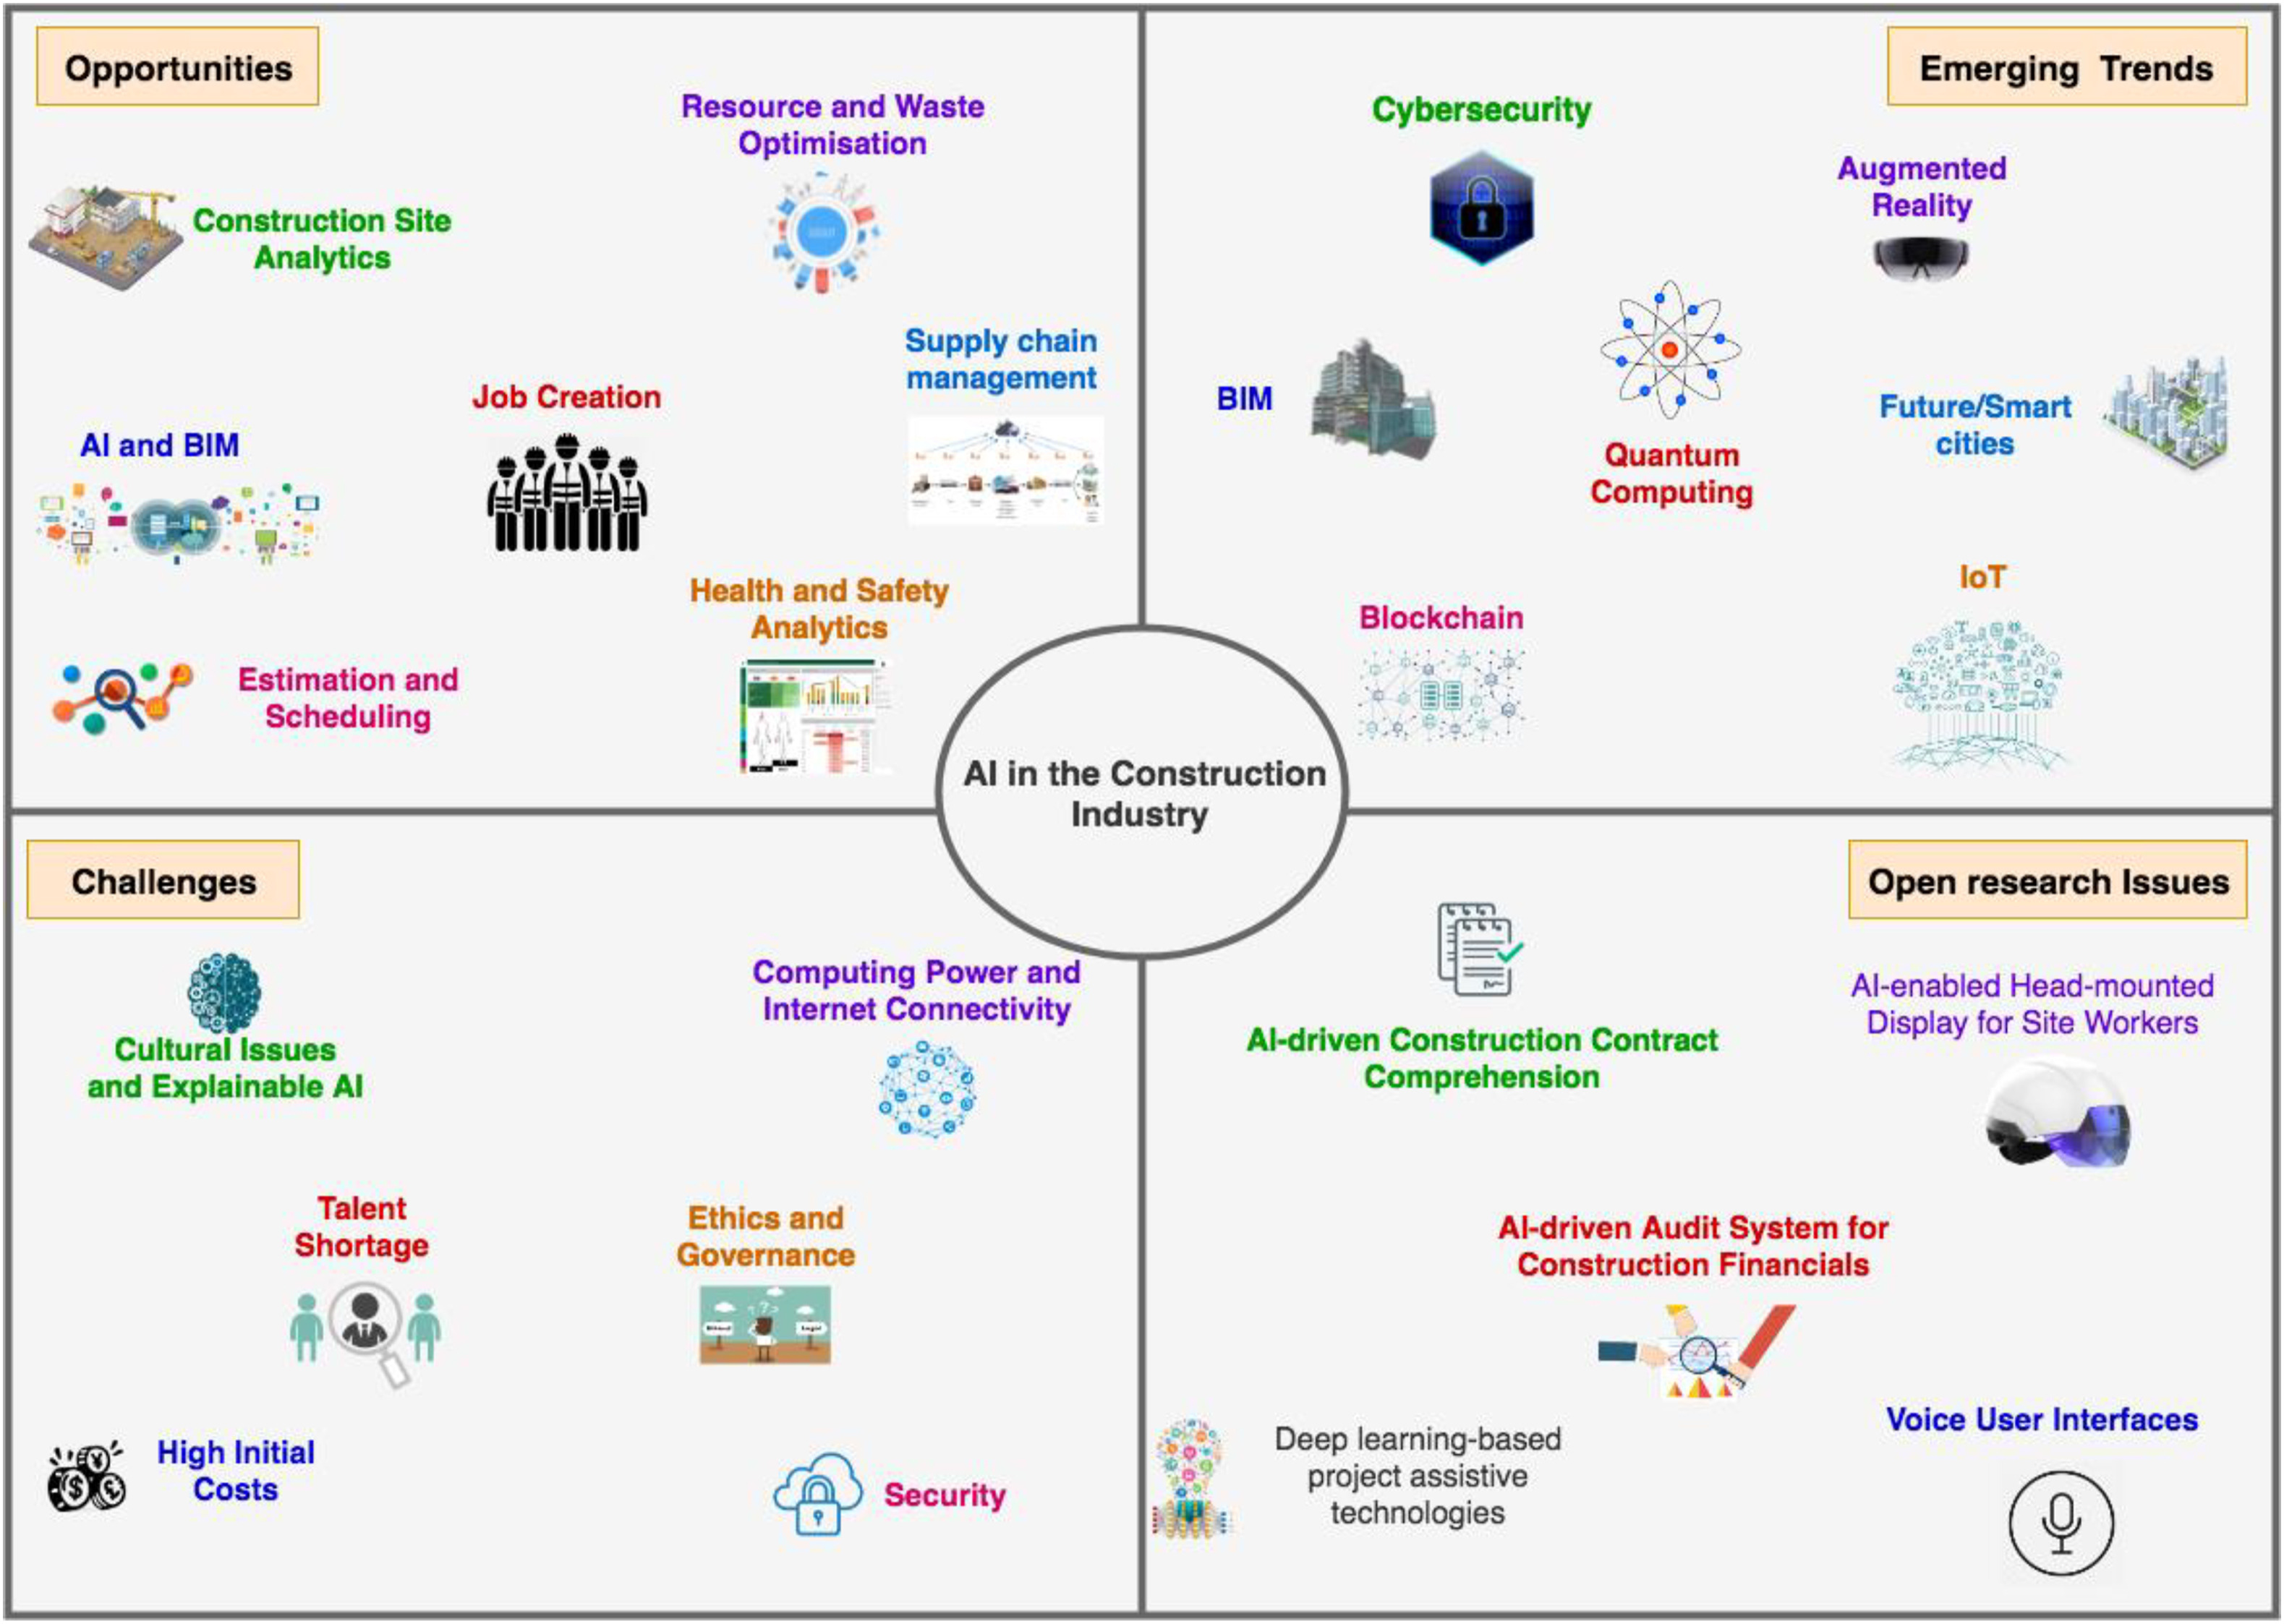
\includegraphics[width=1, height=1\linewidth]{Images/AI in Construction Industry.jpg}
\caption{فرصت ها، روندهای نوظهور، چالش ها و مسائل تحقیقاتی باز}
\label{شکل:AI in Construction Industry}
\end{figure}


\subsection{کمبود استعداد}
در حال حاضر، کمبود جهانی مهندسان هوش مصنوعی با مهارت‌های لازم برای پیشبرد پیشرفت‌های جدی در سراسر صنایع وجود دارد [135]. جذب مهندسان هوش مصنوعی با تجربه در بخش ساخت و ساز برای ساخت راه حل های سفارشی با هدف حل بسیاری از مشکلات در صنعت بسیار دشوار است. این امر را می توان با هزینه بیشتر دولت برای آموزش علوم، فناوری، مهندسی، ریاضیات (STEM) کاهش داد. همچنین، کارشناسان ساخت‌وساز برای همکاری با محققان و کارشناسان صنعت در زمینه هوش مصنوعی برای ادغام ایده‌ها و تولد نوآوری‌های جدید که واقعاً نیازهای صنعت ساخت‌وساز را برآورده می‌کنند، مورد نیاز است.

\subsection{هزینه های اولیه بالا}
مزایای راه حل های مبتنی بر هوش مصنوعی در صنعت ساخت و ساز غیرقابل انکار است. با این حال، هزینه های اولیه مورد نیاز برای سرمایه گذاری در چنین راه حل های هوش مصنوعی به عنوان مثال. رباتیک معمولاً بسیار بالا است. الزامات نگهداری چنین راه حل هایی نیز باید در نظر گرفته شود. این ممکن است برای اکثریت قریب به اتفاق پیمانکاران فرعی و شرکت های کوچک که بخش عمده ای از صنعت ساخت و ساز را تشکیل می دهند غیرقابل تحمل باشد [1]. بنابراین، برای شرکت ها مهم است که صرفه جویی در هزینه و بازگشت سرمایه چنین فناوری هایی را تعیین کنند تا مشخص کنند که آیا سرمایه گذاری کنند یا خیر. علاوه بر این، با پذیرفته شدن و رایج شدن این فناوری ها در ساخت و ساز، انتظار می رود قیمت ها کاهش یابد و برای شرکت های کوچکتر مقرون به صرفه باشد.

\subsection{اخلاق و حکمرانی}
وینفیلد و جیروتکا [136] توضیح دادند که ایجاد و حفظ اعتماد عمومی به فناوری‌های هوش مصنوعی به یک حکومت فراگیر، شفاف و چابک بستگی دارد. این موضوع بسیار مهمی است که برای کل جامعه اهمیت زیادی دارد. شایستگی‌های فناوری‌های هوش مصنوعی در حالی که نوید خروجی‌های عالی را می‌دهد، اگر به درستی تنظیم نشود، می‌تواند خطرناک باشد. به عنوان مثال، یک ربات ساخت و ساز بزرگ که در یک محل ساخت و ساز شلوغ با تعداد زیادی کارگر دچار اختلال می شود و باید سقوط کند. ربات چگونه تصمیم می گیرد که به چپ یا راست بیفتد، بسته به تعداد کارگران در هر طرف، به خوبی می داند که می تواند به معنای مرگ کارگران باشد؟ استفاده از برخی راه‌حل‌های هوش مصنوعی همچنین می‌تواند منجر به مزیت ناعادلانه برای برخی از شرکت‌های صنعت ساخت‌وساز شود که نیاز به تنظیم مقررات دارد.

\subsection{قدرت محاسباتی و اتصال به اینترنت}
سایت های ساخت و ساز عمدتاً از راه دور هستند و فاقد اتصال برق، مخابرات و اینترنت هستند [139]. گاهی اوقات حتی فعالیت های ساختمانی منجر به قطع برق و اتصال به اینترنت می شود. این یک مشکل جدی در استفاده از ابزارهای هوش مصنوعی در سایت‌های ساختمانی ایجاد می‌کند که عملکرد آنها بیشتر به اتصال خوب اینترنت و منبع تغذیه متکی است، به عنوان مثال. روبات ها، سیستم های نظارت بر سایت و غیره [139]. به عنوان مثال، حسگرها و محرک ها اطلاعاتی را که باید در زمان ساخت و ساز در زمان واقعی محاسبه شوند، با یکدیگر ارتباط برقرار می کنند. مناسب است که به دنبال راه هایی برای حل موثر و موثر این مشکل باشید. استفاده از فناوری های ارتباطی 4G (LTE/max) توانسته این مشکل را تا حد قابل توجهی حل کند. ظهور 5G به دلیل سرعت بالای داده، کاهش تاخیر، صرفه جویی در مصرف انرژی، کاهش هزینه، ظرفیت سیستم بالاتر و اتصال گسترده دستگاه، قابلیت اطمینان بیشتری را برای سایت های ساخت و ساز ارائه می دهد.

\section{نتیجه گیری}
هوش مصنوعی به‌عنوان رویکردی نوآورانه برای بهبود بهره‌وری و حل چالش‌ها، آماده است تا تأثیر فوق‌العاده‌ای بر نحوه انجام کارها در چندین صنعت بگذارد. صنعت ساخت‌وساز با مشکل بهره‌وری و چالش‌های بی‌شمار دیگری مواجه است که این پتانسیل را دارد که توسط هوش مصنوعی حل شود. با افزایش داده های تولید شده در طول چرخه عمر ساختمان و ظهور سایر فناوری های دیجیتال، هوش مصنوعی این قابلیت را دارد که از این داده ها استفاده کند و از توانایی های سایر فناوری ها برای بهبود فرآیندهای ساخت و ساز استفاده کند. برای پرداختن به سؤالات تحقیق در این مطالعه، میزان استفاده از فناوری های هوش مصنوعی در ساخت و ساز را بررسی کرده ایم. ما نه تنها آخرین تحقیقات، بلکه تحقیقات مرتبطی را که در شش دهه گذشته در چندین زمینه کاربردی ساخت و ساز منتشر شده است، بررسی کرده ایم. مفاهیم، انواع، مؤلفه ها و زیرشاخه های هوش مصنوعی به اختصار توضیح داده شده و آثار با استفاده از این زیرشاخه ها توضیح داده شده است. خلاصه‌ای اساسی از حوزه‌های کاربردی، مزایا، محدودیت‌ها و مزایای هر زیر شاخه از هوش مصنوعی مورد استفاده در ساخت‌وساز ارائه شد.
این مطالعه یک رویکرد کیفی را از طریق بررسی روند انتشار برای هوش مصنوعی و زیرشاخه‌های آن اتخاذ کرد. جستجوی پایگاه داده با استفاده از جستجوهای پایگاه داده SCOPUS انجام شد و با داده های سه پایگاه داده مجلات دیجیتالی دیگر از جمله Science Direct، IEEE و ACM طی شش دهه (1960-2020) اعتبارسنجی شد.
این پایگاه‌های اطلاعاتی بر اساس استحکام و یکپارچگی آن‌ها و با هدف کاهش سوگیری انتخاب شدند. از داده‌های جمع‌آوری‌شده، زیرشاخه‌های هوش مصنوعی به زمینه‌های نوظهور، رسیده و بالغ در تحقیقات ساخت‌وساز طبقه‌بندی می‌شوند. یافته‌های این مطالعه نشان می‌دهد که بینایی کامپیوتر، رباتیک و NLP تحت فناوری‌های نوظهور قرار می‌گیرند. ML، برنامه‌ریزی و زمان‌بندی خودکار فناوری‌های رسیده هستند در حالی که KBS و بهینه‌سازی فناوری‌های بالغ هستند. بر این اساس، یک چرخه هایپ طراحی و برای پیش‌بینی مدت زمان بلوغ هر فرعی مورد استفاده قرار گرفت. این مطالعه نشان می دهد که در حالی که چندین فناوری هوش مصنوعی در تحقیقات ساخت و ساز به کار گرفته شده است، پیشرفت های اخیر در آن فناوری ها به طور قابل توجهی بهبود یافته است و پذیرش فناوری هوش مصنوعی جدید و قدرتمندتر نسبتا کند بوده است. به عنوان مثال، استفاده از یادگیری عمیق که پتانسیل ارائه پیش بینی های دقیق تری را نسبت به تکنیک های مرسوم ML دارد.
علاوه بر این، این مطالعه برخی فرصت‌ها و موضوعات تحقیقاتی باز را برای تحقیقات هوش مصنوعی در ساخت و ساز شناسایی و مورد بحث قرار داد. اگرچه کاربرد هوش مصنوعی به تدریج در حال افزایش است. ارتباط آن با سایر روندهای نوظهور مانند BIM، IOT، محاسبات کوانتومی، واقعیت افزوده، امنیت سایبری و بلاک چین بیشتر تقویت می شود. ما برخی از چالش‌هایی را که بر پذیرش هوش مصنوعی در صنعت تأثیر می‌گذارد بررسی کردیم و از طریق توصیه‌هایی به آنها پرداختیم. این مطالعه منبع اطلاعات مفیدی برای محققان و متخصصان با توجه به کاربردهای هوش مصنوعی مرتبط و تحقیقات در صنعت ساخت و ساز است. درک روشنی از فرصت ذاتی و همچنین موانع بالقوه زیرشاخه های کاربردی در این مطالعه ارائه شد. ذینفعان ساخت و ساز مانند نهادهای نظارتی، تصمیم گیرندگان، کارگران با مهارت بالا و علاقه مندان به دیجیتال می توانند از اطلاعات ارائه شده در این مطالعه برای تعریف واضح مسیری برای اجرای هوش مصنوعی و کاهش خطرات احتمالی استفاده کنند.




%مراجع و منابع مقاله

\section*{References}
[1] M. Chui, S. Francisco, Artificial Intelligence the Next Digital frontier?., s.L, McKinsey and Company Global Institute, 2017.
[2] D. Young, K. Panthi, O. Noor, Challenges involved in adopting BIM on the construction jobsite, EPiC Series in Built Environment 2 (2021) 302–310. 
[3] J.M.D. Delgado, L. Oyedele, Digital Twins for the built environment: learning from conceptual and process models in manufacturing, Adv. Eng. Inf. 49 (2021), 101332. 
[4] S.A. Bello, L.O. Oyedele, O.O. Akinade, M. Bilal, J.M.D. Delgado, L.A. Akanbi, A. O. Ajayi, H.A. Owolabi, Cloud computing in construction industry: use cases, benefits and challenges, Autom. ConStruct. 122 (2021), 103441. 
[5] A. Nikas, A. Poulymenakou, P. Kriaris, Investigating antecedents and drivers affecting the adoption of collaboration technologies in the construction industry, Autom. ConStruct. 16 (5) (2007) 632–641. 
[6] J.M.D. Delgado, L. Oyedele, Deep learning with small datasets: using autoencoders to address limited datasets in construction management, Appl. Soft Comput. 112 (2021), 107836. 
[7] C.D.-P.S. Chien, W. Huh, Y. Jang, J. Morrison, Artificial intelligence in manufacturing and logistics systems: algorithms, applications, and case studies, Publication Cover Int. J. Prod. Res. 58 (9) (2020) 2730–2731. 
[8] T. Rao, A. Gaddam, M. Kurni, K. Saritha, Reliance on artificial intelligence, machine learning and deep learning in the Era of industry 4.0, in: Smart Healthcare System Design: Security and Privacy Aspects. s.L., Wiley, 2021. 
[9] X. Yao, J. Zhou, J. Zhang, C.R. Bo¨er, From Intelligent Manufacturing to Smart Manufacturing for Industry 4.0 Driven by Next Generation Artificial Intelligence and Further on, 5th International Conference on Enterprise Systems, Beijing, 2017 (ES). 
[10] S.A. Ganiyu, L.O. Oyedele, O. Akinade, H. Owolabi, L. Akanbi, A. Gbadamosi, BIM competencies for delivering waste-efficient building projects in a circular economy, Develop. Built Environ. 4 (2020), 100036. 
[11] A. Ajayi, L. Oyedele, O. Akinade, M. Bilal, H. Owolabi, L. Akanbi, J.M.D. Delgado, Optimised big data analytics for health and safety hazards prediction in power infrastructure operations, Saf. Sci. 125 (2020), 104656. 
[12] A. Khobragade, N. Maheswari, M. Sivagami, Analyzing the housing rate in a real estate informative 
system: a prediction analysis, Int. J. Civ. Eng. Technol. 9 (5) (2018) 1156–1164. 
[13] C. Poh, C.U. Ubeynarayana, Y.M. Goh, Safety leading indicators for construction sites: a machine learning approach, Autom. ConStruct. 93 (2018) 375–386. 
[14] C. Chen, et al., Optimal facility layout planning for AGV-based modular prefabricated manufacturing system, Autom. ConStruct. 98 (2019) 310–321. 
[15] A. Ajayi, L. Oyedele, H. Owolabi, O. Akinade, M. Bilal, J.M.D. Delgado, L. Akanbi, Deep learning models for health and safety risk prediction in power infrastructure projects, Risk Anal. 40 (10) (2020) 2019–2039. 
[16] B. Chu, K. Jung, C. Han, D. Hong, 2010. A survey of climbing robots: Locomotion and adhesion, Int. J. Precis. Eng. Manuf. 11 (4) (2010) 633–647. 
[17] S. Sepasgozar, S. Davis, M. Loosemore, Dissemination practices of construction sites’ Technology Vendors in Technology Exhibitions, J. Manag. Eng. 34 (6) (2018), 04018038, 34(6). 
[18] J.M.D. Delgado, L. Oyedele, A. Ajayi, L. Akanbi, O. Akinade, M. Bilal, H. Owolabi, Robotics and automated systems in construction: understanding industry-specific challenges for adoption, Journal of Building Engineering 26 (2019), 100868. 
[19] E. Shahvand, M.H. Sebt, M.T. Banki, Developing fuzzy expert system for supplier and subcontractor evaluation in construction industry, Scientia Iranica. Transaction A, Civil Engineering 23 (3) (2016) 842. 
[20] L.A. Akanbi, A.O. Oyedele, L.O. Oyedele, R.O. Salami, Deep learning model for Demolition Waste Prediction in a circular economy, J. Clean. Prod. 274 (2020), 122843. 
[21] J. McCarthy, What is Artificial Intelligence, s.L, Computer Science Department, Stanford University, 2007. 
[22] B. Buchanan, A (very) brief history of artificial intelligence, AI Mag. 26 (4) (2005) 53. 
[23] A. Turing, Computing machinery and intelligence, Mind 59 (236) (1950) 433–460. 
[24] W. Ertel, Introduction to Artificial Intelligence, second ed., Springer, Weingarton, 2018. 
[25] E. Brynjolfsson, D. Rock, C. Syverson, Artificial intelligence and the modern productivity paradox: a clash of expectations and statistics, in: The Economics of Artificial Intelligence: An Agenda, s.l.:University of Chicago Press, 2018. 
[26] E. Rich, K. Knight, Artificial Intelligence. s.L, McGraw-Hill, New, 1991. 
[27] S. Baum, A. Barrett, R.V. Yampolskiy, Modeling and interpreting expert disagreement about artificial superintelligence, Informatica 41 (7) (2017) 419–428. 
[28] B. Goertzel, P. Wang, A foundational architecture for artificial general intelligence, Advances in Artificial General Intelligence: Concepts, Architect. Algorithms 6 (2007) 36. 
[29] S. Russell, P. Norvig, Artificial Intelligence: a Modern Approach, Pearson Education Limited, Malaysia, 2016. 
[30] S. Kotsiantis, I. Zaharakis, P. Pintelas, Supervised machine learning: a review of classification techniques, Emerging Artif. Intell. Appl. Comput. Eng. 160 (2007) 3–24. 
[31] R. Gentleman, V.J. Carey, Unsupervised machine learning, in: Bioconductor Case Studies, Springer, New York, NY, 2008, pp. 137–157. 
[32] R. Sutton, Introduction: The challenge of reinforcement learning, in: Reinforcement Learning, Springer, Boston, MA, 1992, pp. 1–3. 
[33] Y. LeCun, Y. Bengio, G. Hinton, Deep learning, Nature 521 (7553) (2015) 436.
[34] J. Schmidhuber, Deep learning in neural networks: an overview, Neural Network. 61 (2015) 85–117. 
[35] A.O. Oyedele, A.O. Ajayi, L.O. Oyedele, Machine learning predictions for lost time injuries in power transmission and distribution projects, Machine Learning with Applications 6 (2021), 100158. 
[36] M. Ghallab, D. Nau, P. Traverso, Automated Planning: Theory and Practice. s.L, Elsevier, 2004. 
[37] A. Fukunaga, G. Rabideau, S. Chien, D. Yan, Towards an Application Framework for Automated Planning and Scheduling. s.L, IEEE, 1997, pp. 375–386. 
[38] G. Cortellessa, A.E. Gerevini, D. Magazzeni, I. Serina, Automated planning and scheduling, Intell. Artif. 8 (1) (2014) 55–56. 
[39] J. Kober, J. Peters, Reinforcement learning in robotics: a survey, in: Reinforcement Learning, Springer, Berlin, 2012, pp. 579–610. 
[40] J. Kolodner, An introduction to case-based reasoning, Artif. Intell. Rev. 6 (1) (1992) 3–34. 
[41] H. Nwana, Intelligent tutoring systems: an overview, Artif. Intell. Rev. 4 (4) (1990) 251–277. 
[42] G. Marchionini, B. Shneiderman, Finding facts vs. browsing knowledge in hypertext systems, Computer 21 (1) (1988) 70–80. 
[43] R. Akerkar, P. Sajja, Knowledge-based Systems. s.L, Jones & Bartlett Publishers, 2010. 
[44] M. Bilal, L.O. Oyedele, J. Qadir, K. Munir, S.O. Ajayi, O.O. Akinade, H. A. Owolabi, H.A. Alaka, A. Pasha, Big Data in the construction industry: a review of present status, opportunities, and future trends, Adv. Eng. Inf. 30 (3) (2016) 500–521. 
[45] G. Chowdhury, Natural language processing, Annu. Rev. Inf. Sci. Technol. 37 (1) (2003) 51–89. 
[46] R. Collobert, et al., Natural language processing (almost) from scratch, J. Mach. Learn. Res. 12 (2011) 2493–2537. 
[47] S. Boyd, L. Vandenberghe, Convex optimization. s.L, Cambridge university press, 2004. 
[48] S. Kiranyaz, T. Ince, M. Gabbouj, Multidimensional Particle Swarm Optimization for Machine Learning and Pattern Recognition, Springer, New York, 2014. 
[49] H. H¨affner, C.F. Roos, R. Blatt, Quantum computing with trapped ions, Phys. Rep. 469 (4) (2008) 155–203. 
[50] M. Hirvensalo, Encyclopedia of sciences and religions, in: Quantum Computing, Springer, Dordrecht, 2013, pp. 1922–1926. 
[51] D. Miorandi, S. Sicari, F. De Pellegrini, I. Chlamtac, 2012. Internet of things: Vision, applications and research challenges, Ad Hoc Netw. 10 (7) (2012) 1497–1516. 
[52] C. Wei, Y. Li, Design of Energy Consumption Monitoring and Energy-Saving Management System of Intelligent Building Based on the Internet of Things, Ningbo, IEEE, 2011, pp. 3650–3652. 
[53] X.J. Luo, L.O. Oyedele, A.O. Ajayi, C.G. Monyei, O.O. Akinade, L.A. Akanbi, Development of an IoT-based big data platform for day-ahead prediction of building heating and cooling demands, Adv. Eng. Inf. 41 (2019), 100926. 
[54] R. Zhong, et al., Prefabricated construction enabled by the Internet-of-Things, Autom. ConStruct. 76 (2017) 59–70, 76, pp. 59–70. 
[55] H. Boyes, Cybersecurity and cyber-resilient supply chains, Technol. Innovation Manage. Rev. 5 (4) (2015) 28. 
[56] S. Race, Construction Manager’s BIM Handbook, in: Cyber Security, John Wiley & Sons Ltd, Chichester(West Sussex), 2016, pp. 107–112. 
[57] J.M.D. Delgado, L. Oyedele, P. Demian, T. Beach, A research agenda for augmented and virtual reality in architecture, engineering and construction, Adv. Eng. Inf. 45 (2020), 101122. 
[58] E. Burton, et al., Ethical Considerations in Artificial Intelligence courses.. s.L, 2017 arXiv preprint arXiv:1701.07769. 
[59] J. Micheal, A. Cohn, J.R. Butcher, BlockChain technology, Practical Law The Journal - Litigation 1 (2018) 35–44. 
[60] A. Lanko, N. Vatin, A. Kaklauskas, Application of RFID combined with blockchain technology in logistics of construction materials, in: s.l., EDP Sciences, 2018, p. 3032. 
[61] Z. Ye, M. Yin, L. Tang, H. Jiang, Cup-of-Water Theory: A Review on the Interaction of BIM, IoT and Blockchain during the Whole Building Lifecycle, 2018 (Berlin, s.n). 
[62] A. Mondragon, C.E.C. Mondragon, E.S. Coronado, Exploring the Applicability of Blockchain Technology to Enhance Manufacturing Supply Chains in the Composite Materials Industry, Chiba, IEEE, 2018. 
[63] M. Najafabadi, et al., Deep learning applications and challenges in big data analytics, Journal of Big Data 2 (1) (2015) 1. 
[64] J. Seo, S. Han, S. Lee, H. Kim, Computer vision techniques for construction safety and health monitoring, Adv. Eng. Inf. 29 (2) (2015) 239–251. 
[65] J. Neelamkavil, Automation in the prefab and modular construction industry. s.l, in: 26th Symposium on Construction Robotics ISARC, 2009. 
[66] R. Bogue, What are the prospects for robots in the construction industry? Ind. Robot: Int. J. 45 (1) (2018) 1–6. 
[67] C. Balaguer, M. Abderrahim, Trends in robotics and automation in construction, in: Robotics and Automation in Construction, IntechOpen, 2008. 
[68] M. Alavi, D. Leidner, 1999. Knowledge management systems: issues, challenges, and benefits, Commun. Assoc. Inf. Syst. 1 (1) (1999) 7. 
[69] M. Bates, R.e. Weischedel, Challenges in Natural Language processing.. s.L, Cambridge University Press, 2006. 
[70] R. Roy, S. Hinduja, R. Teti, Recent advances in engineering design optimisation: challenges and future trends, CIRP Annals 57 (2) (2008) 697–715. 
[71] H.a.S.A. 2. Niska, Data Analytics Approach to Create Waste Generation Profiles for Waste Management and Collection, Waste management, 2018. 
[72] V. Ashokkumar, S. Varghese, BIM based 3D model for construction waste quantification, International Research Journal of Engineering and Technology 5 (5) (2018) 3069–3076. 
[73] Z. Liu, M. Osmani, P. Demian, A. Baldwin, A BIM-aided construction waste minimisation framework, Autom. ConStruct. 59 (2015) 1–23. 
[74] W. Lu, et al., Big data in construction waste management: prospects and challenges, Resour. Conserv. Recycl. 141 (2018) 264–272. 
[75] M. Shafiq, J. Matthews, S. Lockley, A study of BIM collaboration requirements and available features in existing model collaboration systems, J. Inf. Technol. Construct. 18 (2013) 148–161. 
[76] J. Lin, M. Golparvar-Fard, Visual Data and Predictive Analytics for Proactive Project Controls on Construction Sites. s.L, Springer, 2018, pp. 412–430. 
[77] K. Han, M. Golparvar-Fard, Potential of big visual data and building information modeling for construction performance analytics: an exploratory study, Autom. ConStruct. 73 (2017) 184–198. 
[78] K. Schwabe, J. Teizer, M. K¨onig, Applying rule-based model-checking to construction site layout planning tasks, Autom. ConStruct. 97 (97) (2019) 205–219. 
[79] M. Uhm, G. Lee, B. Jeon, An analysis of BIM jobs and competencies based on the use of terms in the industry, Autom. ConStruct. 81 (2017) 67–98. 
[80] N. Araújo, L. Cardoso, J.A.F. Brea, A.F. De Araújo, Green jobs: The present and future of the building industry. Evolution analysis, Soc. Sci. 7 (12) (2018) 266. 
[81] PwC, Will robots really steal our jobs? [Online] Available at: https://www.pwc.co .uk/economic-services/assets/international-impact-of-automation-feb-2018.pdf, 2018 [Accessed 2019]. 
[82] D. Zhang, N. Shah, L.G. Papageorgiou, Efficient energy consumption and operation management in a smart building with microgrid, Energy Convers. Manag. 74 (2013) 209–222. 
[83] M. Rathore, A. Ahmad, A. Paul, S. Rho, Urban planning and building smart cities based on the internet of things using big data analytics, Comput. Network. 101 (2016) 63–80. 
[84] B. Balaji, et al., Brick: Metadata schema for portable smart building applications, Appl. Energy 226 (2018) 1273–1292. 
[85] S. Yamamura, L. Fan, Y. Suzuki, Assessment of urban energy performance through integration of BIM and GIS for smart city planning, Procedia Eng. 180 (2017) 1462–1472. 
[86] C. Park, D.Y. Lee, O.S. Kwon, X. Wang, A framework for proactive construction defect management using BIM, augmented reality and ontology-based data collection template, Autom. ConStruct. 33 (2013) 61–71. 
[87] Q. Le, et al., A framework for using mobile based virtual reality and augmented reality for experiential construction safety education, Int. J. Eng. Educ. 31 (3) (2015) 713–725. 
[88] S. Rankohi, L. Waugh, Review and analysis of augmented reality literature for construction industry, Visual. Eng. 1 (1) (2013) 9. 
[89] Y. Tsang, et al., An Internet of Things (IoT)-based risk monitoring system for managing cold supply chain risks, Ind. Manag. Data Syst. 118 (7) (2018) 1432–1462. 
[90] J. Barata, P. Rupino Da Cunha, J. Stal, Mobile supply chain management in the industry 4.0 era: an annotated bibliography and guide for future research, J. Enterprise Inf. Manag. 31 (1) (2018) 173–192. 
[91] W. Xiong, et al., Improving Supply Chain Communications for Off-Site Construction Using Process Specification Language, 2018, pp. 1–9. Berlin, IAARC. 
[92] S. Zhang, et al., BIM-based fall hazard identification and prevention in construction safety planning, Saf. Sci. 72 (2015) 31–45. 
[93] I. Awolusi, E. Marks, M. Hallowell, Wearable technology for personalized construction safety monitoring and trending: Review of applicable devices, Autom. ConStruct. 85 (2018) 96–106. 
[94] A. Sidani, et al., Improving Construction Safety Using BIM-Based Sensor Technologies, ptBIM, lisboa, 2018. 
[95] A. Sidani, et al., The Impact of BIM-based virtual and augmented reality interfaces on health and safety in construction projects: protocol for a systematic review, Int. J. Occup. Environ. Safety 2 (1) (2018) 67–74. 
[96] M. Safa, A. Shahi, C. Haas, K. Hipel, Construction contract management using value packaging systems, Int. J. Construction Manag. 1 (2017) 50–64. 
[97] A. Boonpheng, et al., Blockchain technology and cryptocurrency are databases for contract management in construction engineering, Int. J. Adv. Res. Eng. Technol. 12 (1) (2021) 1073–1084. 
[98] O. Olanrewaju, M. Sandanayake, S. Babarinde, Voice assisted key-in building quantities Estimation system, J. Eng. Proj. Prod. Manag. 10 (2) (2020). 
[99] A. Sheldon, et al., Putting the AR in (AR) chitecture-Integrating voice recognition and gesture control for Augmented Reality interaction to enhance design practice. Wellington, New Zealand, in: Proceedings of the 24th CAADRIA Conference, 2019. 
[100] M. Vigneault, C. Boton, H. Chong, B. Cooper-Cooke, An innovative framework of 5D BIM solutions for construction cost management: a systematic review, Arch. Comput. Methods Eng. 27 (4) (2020) 1013–1030. 
[101] R. Zheng, J. Jiang, X. Hao, W. Ren, F. Xiong, Y. Ren, bcBIM: A Blockchain-Based Big Data Model for BIM Modification Audit and Provenance in Mobile Cloud, Mathematical Problems in Engineering (2019) 1–13, https://doi.org/10.1155/ 2019/5349538, 5349538 In this issue. 
[102] H. Dahlbo, et al., Construction and demolition waste management–a holistic evaluation of environmental performance, J. Clean. Prod. 107 (2015) 333–341. 
[103] N. Shan, S.T. Wee, T.L. Wai, G.K. Chen, Construction waste management of Malaysia: case study in Penang, Adv. Sci. Lett. 24 (6) (2018) 4698–4703, 24(6), pp. 4698–4703.
[104] M. Bilal, L.O. Oyedele, O.O. Akinade, S.O. Ajayi, H.A. Alaka, H.A. Owolabi, J. Qadir, M. Pasha, S.A. Bello, Big data architecture for construction waste analytics (CWA): a conceptual framework, Journal of Building Eng. 6 (2016) 144–156. 
[105] O.O. Akinade, L.O. Oyedele, Integrating construction supply chains within a circular economy: an ANFIS-based waste analytics system (A-WAS), J. Clean. Prod. 229 (2019) 863–873. 
[106] M. Bilal, L.O. Oyedele, K. Munir, S.O. Ajayi, O.O. Akinade, H.A. Owolabi, H. A. Alaka, The application of web of data technologies in building materials information modelling for construction waste analytics, Sustain. Mater. Technol. 11 (2017) 28–37. 
[107] L. Akanbi, L. Oyedele, J.M.D. Delgado, M. Bilal, O. Akinade, A. Ajayi, N. Mohammed-Yakub, Reusability analytics tool for end-of-life assessment of building materials in a circular economy, World J. Sci. Technol. Sustain. Develop. 16 (1) (2019) 40–55. 
[108] S. Azhar, M. Khalfan, T. Maqsood, Building information modelling (BIM): now and beyond, Construct. Econ. Build. 12 (4) (2012) 15–28. 
[109] Z. Lin, A. Chen, S. Hsieh, Temporal image analytics for abnormal construction activity identification, Autom. ConStruct. 124 (2021), 103572. 
[110] A. Ajayi, L. Oyedele, J.M.D. Delgado, L. Akanbi, M. Bilal, O. Akinade, O. Olawale, Big data platform for health and safety accident prediction, World J. Sci. Technol. Sustain. Develop. 16 (1) (2019) 2–21. 
[111] R. Eadie, et al., A survey of current status of and perceived changes required for BIM adoption in the UK, Built. Environ. Proj. Asset. Manag. 5 (2015) 4–21. 
[112] D. Walasek, A. Barszcz, Analysis of the adoption rate of building information modeling [BIM] and its return on investment [ROI], Procedia Eng. 172 (2017) 1227–1234. 
[113] X. Luo, H. Li, D. Cao, F. Dai, Recognizing diverse construction activities in site images via relevance Networks of construction-related objects detected by convolutional Neural Networks, J. Comput. Civ. Eng. 32 (3) (2018). 
[114] L.O. Oyedele, K.W. Tham, Clients’ assessment of architects’ performance in building delivery process: Evidence from Nigeria, Build. Environ. 42 (5) (2007) 2090–2099. 
[115] S.O. Ajayi, L.O. Oyedele, M. Bilal, O.O. Akinade, H.A. Alaka, H.A. Owolabi, Critical management practices influencing on-site waste minimization in construction projects, Waste Manag. 59 (2017) 330–339. 
[116] S. Winge, E. Albrechtsen, B.A. Mostue, Causal factors and connections in construction accidents, Saf. Sci. 112 (2019) 130–141. 
[117] A. Oyedele, A. Ajayi, L. Oyedele, J.M.D. Delgado, L. Akanbi, O. Akinade, H. Owolabi, M. Bilal, Deep learning and Boosted trees for injuries prediction in power infrastructure projects, Appl. Soft Comput. 110 (2021) 107587. 
[118] K. Muhammad, O. Saoula, M. Issa, U. Ahmed, Contract management and performance characteristics: an empirical and managerial implication for Indonesia, Manage. Sci. Letters 9 (8) (2019) 1289–1298. 
[119] T. Nguyen, et al., MS MARCO: A Human Generated Machine Reading Comprehension Dataset, Microsoft AI & Research, Barcelona, Spain, 2016. 
[120] A. Trischler, et al., Newsqa: A Machine Comprehension Dataset, s.l., s.n, 2016. 
[121] G. L´opez, L. Quesada, L.A. Guerrero, Alexa vs. Siri vs. Cortana vs. Google Assistant: a Comparison of Speech-Based Natural User Interfaces. s.L, Springer, Cham, 2017, pp. 241–250. 
[122] S. Xia, J. Nie, X. Jiang, CSafe: an intelligent audio wearable platform for improving construction worker safety in urban Environments. s.l, in: Proceedings of the 20th International Conference on Information Processing in Sensor Networks (Co-located with CPS-IoT Week 2021), 2021, pp. 207–221. 
[123] H. Alaka, L.O. Oyedele, H.A. Owolabi, O.O. Akinade, M. Bilal, S.O. Ajayi, A Big Data analytics approach for construction firms failure prediction models, IEEE Trans. Eng. Manag. 66 (4) (2018) 689–698. 
[124] Y. Jang, I. Jeong, Y. Cho, Identifying impact of variables in deep learning models on bankruptcy prediction of construction contractors, Eng. Construct. Architect. Manag. 28 (2021). 
[125] H. Alaka, L.O. Oyedele, H.A. Owolabi, M. Bilal, S.O. Ajayi, O.O. Akinade, Insolvency of small civil engineering firms: critical strategic factors, ASCE J. Profession. Issues Eng. Educ. Pract. 143 (3) (2017), 04016026. 
[126] M. Bilal, Oyedele, Big Data with deep learning for benchmarking profitability performance in project tendering, Expert Syst. Appl. 147 (2020), 113194. 
[127] H. Alaka, L.O. Oyedele, H.A. Owolabi, A.O. Oyedele, O.O. Akinade, M. Bilal, S. O. Ajayi, Critical factors for insolvency prediction: towards a theoretical model for the construction industry, Int. J. Construct. Manage. 17 (1) (2017) 25–49. 
[128] H. Alaka, L.O. Oyedele, H.A. Owolabi, K. Vikas, S.O. Ajayi, O.O. Akinade, M. Bilal, Systematic review of bankruptcy prediction models: Towards a framework for tool selection, Expert Syst. Appl. 94 (2018) 164–184. 
[129] M. Bilal, L.O. Oyedele, H.O. Kusimo, H.A. Owolabi, L.A. Akanbi, A.O. Ajayi, O. O. Akinade, J.M.D. Delgado, Investigating profitability performance of construction projects using big data: a project analytics approach, J. Build. Eng. 26 (2019), 100850. 
[130] M. Ribeiro, S. Singh, C. Guestrin, Why Should I Trust You?: Explaining the Predictions of Any Classifier, California, San Francisco, 2016, pp. 1135–1144. ACM. 
[131] A. Binder, et al., Layer-wise Relevance Propagation for Neural Networks with Local Renormalization Layers, Springer, Barcelona, 2016, pp. 63–71. 
[132] J. Frank, Artificial intelligence and intrusion detection: current and future directions. s.l, in: Proceedings of the 17th National Computer Security Conference, 1994, pp. 1–12. 
[133] L.O. Oyedele, B.E. Jaiyeoba, K.O. Kadiri, S.O. Folagbade, I.K. Tijani, R.O. Salami, Critical factors affecting construction quality in Nigeria: evidence from industry professionals, Int. J. Sustain. Build. Technol. Urban Develop. 6 (2) (2015) 103–113. 
[134] L. Huang, et al., Adversarial Machine Learning, ACM, Chicago, Illinois, 2011, pp. 43–58. 
[135] EY and MIT Technology Review Insights, The Growing Impact of AI on Business [Acces, 2018 [Online] Available at: https://www.ey.com/Publication/vwLUAsset s/ey-ai-creates-jobs-yet-talent-crisis-remains/$File/ey-ai-creates-jobs-yet-talent-c risis-remains.pdf.
[136] A. Winfield, M. Jirotka, Ethical governance is essential to building trust in robotics and artificial intelligence systems, Phil. Trans. R. Soc. A 376 (2133) (2018), 20180085. 
[137] H. Yu, et al., Building Ethics into artificial intelligence. s.l, in: IJCAI, 2018, pp. 5527–5533. 
[138] R. Yampolskiy, Artificial intelligence safety engineering: Why machine ethics is a wrong approach, in: Philosophy and Theory of Artificial Intelligence, Springer, Berlin, Heidelberg, 2013, pp. 389–396. 
[139] J. Louis, P. Dunston, Integrating IoT into operational workflows for real-time and automated decision-making in repetitive construction operations, Autom. ConStruct. 94 (2018) 317–327. 
[140] A. Gbadamosi, et al., A BIM Based Approach for Optimization of Construction and Assembly through Material Selection, Slovenia, Ljubljana, 2018. 
[141] A. Gbadamosi, et al., Offsite construction: developing a BIM-based optimizer for assembly, J. Clean. Prod. 215 (2019) 1180–1190. 
[142] M. Zaher, D. Greenwood, M. Marzouk, Mobile augmented reality applications for construction projects, Construct. Innovat. 18 (2) (2018) 152–166, 18(2), pp. 152–166.





\bibliography{lib}

\theendnotes
\end{document}

